\documentclass[11pt,a4paper]{report}
\newcommand{\TanggalLaporan}{22 November 2026}
% Sengaja kosong sesuai arahan anggota kelompok; jangan menyalin kontribusi M1.
\newcommand{\KontribusiAzka}{}
\newcommand{\KontribusiArlow}{}
\newcommand{\KontribusiFachriza}{}

\usepackage[utf8]{inputenc}
\input{glyphtounicode}
\pdfgentounicode=1
\usepackage[T1]{fontenc}
\usepackage[a4paper,margin=2.4cm,headheight=15pt]{geometry}
\usepackage{lmodern,parskip,enumitem,graphicx,caption}
\usepackage{booktabs,array,tabularx,longtable,amsmath}
\usepackage{xcolor,listings,tikz}
\usetikzlibrary{arrows.meta,positioning,fit,backgrounds,calc}
\usepackage{xurl}
\usepackage[hidelinks]{hyperref}
\usepackage{fancyhdr}
\definecolor{reportblue}{HTML}{214C68}
\definecolor{reportlight}{HTML}{EDF4F7}
\definecolor{reportorange}{HTML}{AD5620}
\definecolor{codebg}{HTML}{F4F5F6}
\hypersetup{pdftitle={IF4031 M2 - ARLOW - nasigoreng},pdfauthor={Kelompok nasigoreng},pdfsubject={Laporan implementasi dan bukti Milestone 2}}
\pagestyle{fancy}\fancyhf{}
\fancyhead[L]{\small IF4031 -- ARLOW / nasigoreng}
\fancyhead[R]{\small\nouppercase{\leftmark}}
\fancyfoot[C]{\thepage}
\renewcommand{\chaptermark}[1]{\markboth{Bab \thechapter}{}}
\setlength{\emergencystretch}{3em}
\setlength{\tabcolsep}{4pt}
\renewcommand{\arraystretch}{1.18}
\setlist{nosep,topsep=5pt,leftmargin=*}
\setcounter{tocdepth}{1}
\lstset{basicstyle=\ttfamily\footnotesize,backgroundcolor=\color{codebg},breaklines=true,columns=fullflexible,keepspaces=true,showstringspaces=false,frame=single,rulecolor=\color{black!15},aboveskip=8pt,belowskip=8pt}
\DeclareRobustCommand{\code}[1]{\nolinkurl{#1}}
\newcolumntype{P}[1]{>{\raggedright\arraybackslash}p{#1}}
\newcolumntype{Y}{>{\raggedright\arraybackslash}X}
\renewcommand{\contentsname}{Daftar Isi}
\renewcommand{\chaptername}{Bab}
\renewcommand{\figurename}{Gambar}
\renewcommand{\tablename}{Tabel}
\renewcommand{\bibname}{Daftar Pustaka}
\renewcommand{\appendixname}{Lampiran}
\newcommand{\bukti}[1]{\textbf{[#1]}}
\newcommand{\sumber}[1]{\par\smallskip{\footnotesize\textit{Dasar penelusuran:} #1}\par}
\tikzset{box/.style={draw=reportblue,rounded corners=3pt,fill=reportlight,align=center,font=\small,inner sep=7pt},arr/.style={-{Stealth[length=2mm]},thick,draw=reportblue}}

\begin{document}
\hypersetup{pageanchor=false}
\begin{titlepage}
\centering
{\Large Tugas Besar IF4031\\[.2cm]Arsitektur Aplikasi Terdistribusi\par}
\vspace{2.3cm}
{\Huge\bfseries\color{reportblue} ARLOW\par}
\vspace{.4cm}
{\LARGE\bfseries Agregasi Real-time\\Layanan Operasi Waspada\par}
\vspace{.9cm}
{\Large Laporan Milestone 2\\[.2cm]Sistem Terdistribusi Skalabel\par}
\vspace{.9cm}
\rule{.7\textwidth}{.6pt}\\[.8cm]
{\large Kelompok \textbf{nasigoreng}\par}
\vspace{.7cm}
\begin{tabular}{ll}
Muhammad Aulia Azka & 13523137\\
Arlow Emmanuel Hergara & 13523161\\
Fachriza Ahmad Setiyono & 13523162
\end{tabular}
\vfill
{\large Program Studi Teknik Informatika\\
Sekolah Teknik Elektro dan Informatika\\
Institut Teknologi Bandung\\[.5cm]\TanggalLaporan\par}
\end{titlepage}
\hypersetup{pageanchor=true}
\pagenumbering{roman}
\chapter*{Kontribusi Anggota}
\addcontentsline{toc}{chapter}{Kontribusi Anggota}
\begin{tabularx}{\textwidth}{@{}P{2cm}P{5cm}Y@{}}
\toprule NIM & Nama & Kontribusi Milestone 2\\\midrule
13523137 & Muhammad Aulia Azka & \KontribusiAzka\\\addlinespace
13523161 & Arlow Emmanuel Hergara & \KontribusiArlow\\\addlinespace
13523162 & Fachriza Ahmad Setiyono & \KontribusiFachriza\\\bottomrule
\end{tabularx}
\chapter*{Catatan Cakupan Laporan}
\addcontentsline{toc}{chapter}{Catatan Cakupan Laporan}
Laporan ini menyajikan implementasi dan hasil pengujian M2. Angka hasil pengujian diambil dari artefak tersimpan; hasil lokal dan hasil pada cluster dibedakan pada setiap bab. Pernyataan ``belum terbukti'' berarti bukti yang diperlukan belum tersedia, sedangkan ``target belum tercapai'' berarti hasil yang tersedia memang berada di luar target.

Kode layanan yang diperiksa berada pada commit \code{36303a7}; Aggregator dalam snapshot deployment 18 menggunakan image dari commit \code{d773970}. Komponen lain mengikuti digest masing-masing pada snapshot. Snapshot infrastruktur tersebut adalah \code{4b6f5096eb380f6d09b65fe8824a801919f3061f}. Bukti pengujian dapat berasal dari versi sebelumnya dan identitas versinya dipertahankan pada artefak asal.

Baseline M1 adalah laporan bertanggal 10 Oktober 2026 beserta commit \code{122ca7b} dan bukti \code{4a1973b}.

Form penggunaan AI terdapat pada Lampiran~\ref{app:ai}.
\tableofcontents
\clearpage
\pagenumbering{arabic}
\chapter{Gambaran Sistem dan Deployment}
\section{Tujuan dan Ruang Lingkup}
ARLOW mengubah data kebencanaan dari beberapa instansi menjadi \code{HazardEvent} kanonik, lalu menyediakannya melalui REST, live feed SSE, webhook, dan notifikasi. M1 membuktikan integrasi BMKG/PVMBG, isolasi kegagalan sumber, autentikasi, pemisahan layanan, serta distribusi event. M2 membawa sistem tersebut ke beberapa node, menambah penyimpanan terdistribusi, koordinasi beberapa Aggregator, penerimaan laporan lapangan yang tahan kegagalan, serta sumber satelit dan sensor pantai~\cite{spec,m1}.

Pengguna terdiri atas Media, Tim Lapangan, dan BNPB Internal. Media memperoleh ringkasan sesuai scope; Tim Lapangan dapat mengirim laporan dan menerima peringatan; Internal Ops dapat memeriksa serta memproses ulang pesan gagal dengan scope khusus. Token Audit terpisah dipakai untuk pemeriksaan oleh asisten. Semua data uji merupakan data simulasi.

\section{Arsitektur Logis}
\begin{figure}[htbp]
\centering
\resizebox{\textwidth}{!}{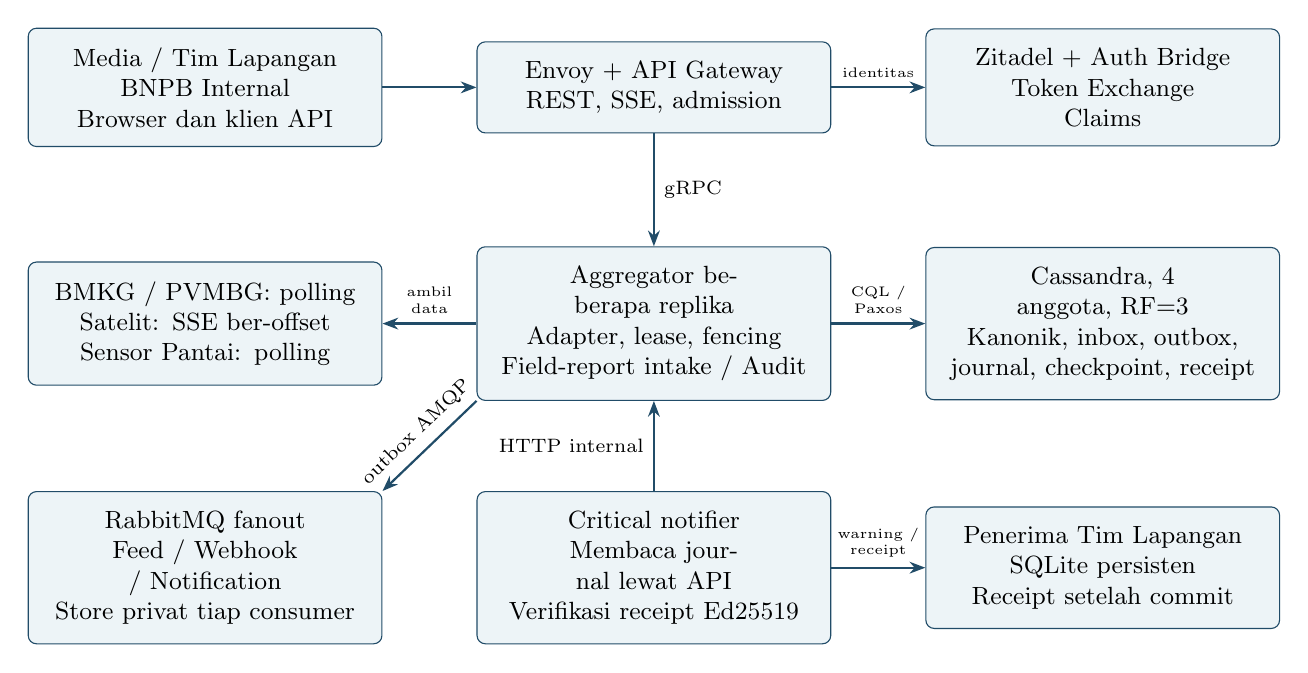
\begin{tikzpicture}
\node[box,text width=4cm] (clients) at (0,0) {Media / Tim Lapangan\\BNPB Internal\\Browser dan klien API};
\node[box,text width=4cm] (edge) at (5.7,0) {Envoy + API Gateway\\REST, SSE, admission};
\node[box,text width=4cm] (auth) at (11.4,0) {Zitadel + Auth Bridge\\Token Exchange\\Claims};
\node[box,text width=4cm] (sources) at (0,-3) {BMKG / PVMBG: polling\\Satelit: SSE ber-offset\\Sensor Pantai: polling};
\node[box,text width=4cm] (agg) at (5.7,-3) {Aggregator beberapa replika\\Adapter, lease, fencing\\Field-report intake / Audit};
\node[box,text width=4cm] (store) at (11.4,-3) {Cassandra, 4 anggota, RF=3\\Kanonik, inbox, outbox,\\journal, checkpoint, receipt};
\node[box,text width=4cm] (broker) at (0,-6.1) {RabbitMQ fanout\\Feed / Webhook / Notification\\Store privat tiap consumer};
\node[box,text width=4cm] (critical) at (5.7,-6.1) {Critical notifier\\Membaca journal lewat API\\Verifikasi receipt Ed25519};
\node[box,text width=4cm] (receiver) at (11.4,-6.1) {Penerima Tim Lapangan\\SQLite persisten\\Receipt setelah commit};
\draw[arr] (clients) -- (edge);
\draw[arr] (edge) -- node[above,font=\tiny]{identitas} (auth);
\draw[arr] (edge) -- node[right,font=\scriptsize]{gRPC} (agg);
\draw[arr] (agg) -- node[above,font=\tiny,align=center]{ambil\\data} (sources);
\draw[arr] (agg) -- node[above,font=\tiny,align=center]{CQL /\\Paxos} (store);
\draw[arr] (agg.south west) -- node[above,sloped,font=\scriptsize]{outbox AMQP} (broker.north east);
\draw[arr] (critical) -- node[left,font=\scriptsize]{HTTP internal} (agg);
\draw[arr] (critical) -- node[above,font=\tiny,align=center]{warning /\\receipt} (receiver);
\end{tikzpicture}}
\caption{Arsitektur M2. Panah menunjukkan arah pemanggilan/pengiriman; jawaban mengalir kembali. Telemetri seluruh jalur dikumpulkan oleh OpenTelemetry dan Grafana LGTM. Diagram dibuat dari kode dan konfigurasi, bukan tangkapan layar runtime.}
\label{fig:architecture}
\end{figure}

Envoy menyediakan pintu masuk publik. Token Exchange menjalankan \code{ext_authz} dan pertukaran token ke Zitadel; API Gateway menerjemahkan HTTP menjadi gRPC dan membatasi konkurensi. Layanan bisnis memverifikasi identitas/scopes. Pembacaan hazard memakai penyimpanan BNPB sehingga permintaan client tidak memanggil sumber yang sedang bermasalah secara sinkron.

Setiap job pengambilan sumber mempunyai lease sendiri. Semua replika Aggregator melayani pembacaan, tetapi satu term yang berwenang menjalankan job sumber tertentu. Cassandra menyimpan event, otoritas penulis, journal input, checkpoint, inbox gagal, serta keadaan pengiriman. SQLite privat pada pemroses satelit hanyalah keadaan kerja turunan; sumber pemulihannya tetap journal dan snapshot di Cassandra.

Publikasi biasa melalui outbox dan RabbitMQ menuju tiga consumer independen. Jalur kritis memiliki journal immutable tambahan: notifier mengambilnya melalui API Aggregator, mengirim byte yang sama ke penerima Tim Lapangan, lalu menyimpan receipt bertanda tangan. ACK broker atau FCM tidak dipakai sebagai bukti bahwa penerima telah menerima peringatan.
\sumber{\code{services/README.md}; \code{docs/m2-write-authority.md}; \code{docs/m2-critical-delivery.md}; kode adapter, storage, dan gateway pada manifest sumber.}

\section{Teknologi Terpilih}
\begin{longtable}{@{}P{3.1cm}P{3.4cm}P{8.9cm}@{}}
\toprule Komponen & Teknologi & Alasan dan peran\\\midrule\endhead
Aggregator dan worker & Go, gRPC & Mempertahankan implementasi M1; konkurensi job, stream, RPC, dan worker terpisah dengan konteks pembatalan.\\
Penyimpanan kanonik & Cassandra 5.0.9, RF=3, Paxos v2 & Partisi, replikasi, pembacaan quorum dan conditional write; konsekuensinya koordinasi lintas node menambah latensi. PostgreSQL tetap backend alternatif pengembangan.\\
Satelit & Go, SQLite keadaan kerja & Graf deteksi disimpan di disk agar payload besar tidak memaksa seluruh graf tinggal di heap; snapshot/journal direplikasi di canonical store.\\
Event Live Feed & Rust, Redis & Streaming asinkron; replay lintas restart dengan buffer persisten berbatas.\\
Webhook / Notification & Go / .NET 10; PostgreSQL, Redis sesuai layanan & Penyimpanan langganan, status delivery, deduplikasi dan push outbox tidak berbagi tabel kanonik.\\
Mock sumber & Python, SQLite & Mock BMKG/PVMBG tetap mandiri; PVMBG menambah mode skema tidak kompatibel.\\
Identitas dan edge & Zitadel, Node.js Auth Bridge, Rust sidecar, Envoy & Mempertahankan OIDC, cookie sesi, pertukaran token, role dan scope M1.\\
Frontend & React, TypeScript, nginx & Daftar/detail/live hazard dan dashboard analitik lintas katalog.\\
Broker & RabbitMQ 4, AMQP, Protobuf & Fanout, confirmation, acknowledgement, dan queue consumer independen.\\
Platform & k3s, Calico, Helm, Flux, SOPS/age & Kernel node terpisah, policy jaringan, konfigurasi deklaratif dan snapshot deployment.\\
Observabilitas / uji & OpenTelemetry, Grafana LGTM, k6 & Trace, metrik dan log berkorelasi; pembebanan HTTP dari luar pod aplikasi.\\\bottomrule
\end{longtable}

\section{Deklarasi Topologi dan Penempatan}
Empat node k3s berjalan dengan empat kernel Linux terpisah pada tiga host fisik \bukti{E01,E02}.

\begin{longtable}{@{}P{1.5cm}P{4.2cm}P{3.3cm}P{6.3cm}@{}}
\toprule Node & Peran dan jenis guest & Kapasitas guest & Host fisik dan spesifikasi\\\midrule\endhead
\code{bnpb-a} & Control plane + worker; Ubuntu 22.04 WSL2 VM & 8 vCPU; 5,8 GiB & ROG-RIZA, Windows 11; Ryzen 9 6900HS, 8 core/16 thread; RAM 16 GB (15,24 GiB terlapor).\\
\code{bnpb-b} & Worker; Ubuntu 26.04 QEMU VM & 2 vCPU; 5,8 GiB & Linux-BC, Gentoo; 4 core/8 thread; RAM 16 GB.\\
\code{bnpb-c} & Worker; Ubuntu 26.04 QEMU VM & 2 vCPU; 5,8 GiB & Linux-BC, Gentoo; 4 core/8 thread; RAM 16 GB.\\
\code{bnpb-d} & Worker; Ubuntu 24.04 WSL2 VM & 16 vCPU; 7,6 GiB & Windows-11-D, Windows 11; 8 core/16 thread; RAM 16 GB.\\\bottomrule
\end{longtable}

Kapasitas guest merupakan alokasi/kapasitas yang terlihat oleh Kubernetes, bukan penjumlahan kapasitas fisik tambahan. Jaringan antar-node memakai Tailscale dan Calico VXLAN dengan MTU pod 1230. Versi k3s pada pengamatan akhir adalah \code{v1.34.13+k3s1}. Empat node akhir berstatus Ready. Kendali HPA Aggregator kembali pada minimum 3 dan maksimum 5; pengamatan akhir memuat empat pod Aggregator berjalan. Skenario gangguan diarahkan ke worker non-control-plane.

\begin{figure}[p]
\centering
\resizebox{\textwidth}{!}{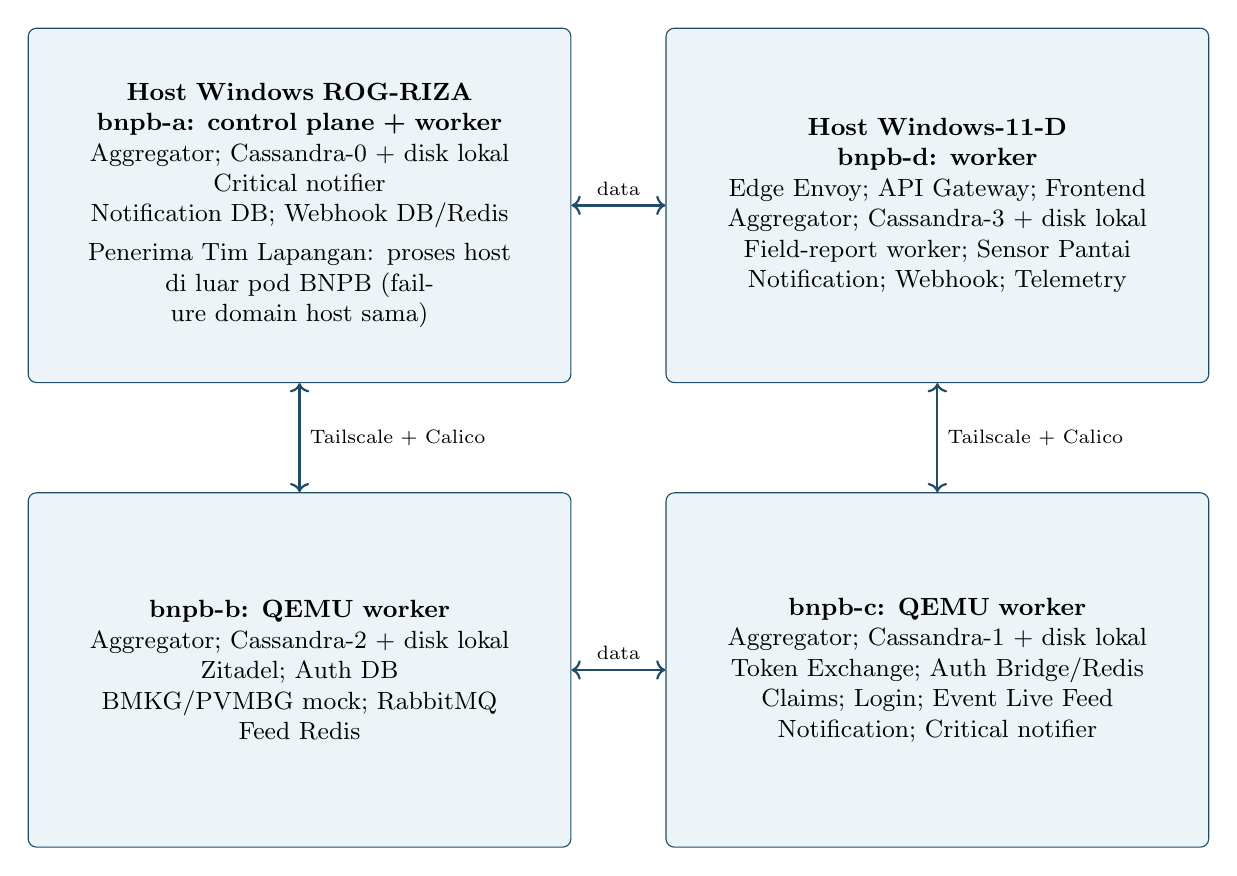
\begin{tikzpicture}
\node[box,text width=6.4cm,minimum height=4.5cm] (a) at (0,0) {\textbf{Host Windows ROG-RIZA}\\\textbf{bnpb-a: control plane + worker}\\Aggregator; Cassandra-0 + disk lokal\\Critical notifier\\Notification DB; Webhook DB/Redis\\\smallskip Penerima Tim Lapangan: proses host\\di luar pod BNPB (failure domain host sama)};
\node[box,text width=6.4cm,minimum height=4.5cm] (d) at (8.1,0) {\textbf{Host Windows-11-D}\\\textbf{bnpb-d: worker}\\Edge Envoy; API Gateway; Frontend\\Aggregator; Cassandra-3 + disk lokal\\Field-report worker; Sensor Pantai\\Notification; Webhook; Telemetry};
\node[box,text width=6.4cm,minimum height=4.5cm] (b) at (0,-5.9) {\textbf{bnpb-b: QEMU worker}\\Aggregator; Cassandra-2 + disk lokal\\Zitadel; Auth DB\\BMKG/PVMBG mock; RabbitMQ\\Feed Redis};
\node[box,text width=6.4cm,minimum height=4.5cm] (c) at (8.1,-5.9) {\textbf{bnpb-c: QEMU worker}\\Aggregator; Cassandra-1 + disk lokal\\Token Exchange; Auth Bridge/Redis\\Claims; Login; Event Live Feed\\Notification; Critical notifier};
\draw[arr,<->] (a) -- node[above,font=\scriptsize]{data} (d);
\draw[arr,<->] (b) -- node[above,font=\scriptsize]{data} (c);
\draw[arr,<->] (a) -- node[right,font=\scriptsize]{Tailscale + Calico} (b);
\draw[arr,<->] (d) -- node[right,font=\scriptsize]{Tailscale + Calico} (c);
\end{tikzpicture}}
\caption{Penempatan komponen utama pada pengamatan akhir 22 November \bukti{E02}; lokasi edge dan receiver dilengkapi dari bukti diagnosis serta konfigurasi receiver. Panah merangkum jalur jaringan antar-node, bukan pembatas bahwa koneksi hanya boleh mengikuti sisi kotak. Job migrasi/debug sementara tidak ditampilkan. Penempatan dapat berubah karena scheduler/HPA.}
\label{fig:deployment}
\end{figure}

Replikasi Cassandra menoleransi satu anggota hilang selama dua dari tiga replika tiap partisi tetap tersedia. Hal ini tidak menjamin quorum bila seluruh host Linux-BC yang memuat dua anggota mati. Receiver Tim Lapangan pada host a berada di luar pod/worker sasaran b atau c, tetapi belum merupakan perangkat fisik terpisah dari seluruh host BNPB. Auth DB, broker dan beberapa store layanan juga belum ditunjukkan memiliki toleransi kehilangan host setara canonical store.

\section{Kontrak Platform, Sumber Daya, dan Isolasi}
Namespace aplikasi adalah \code{sistem-informasi-kebencanaan-bnpb}. Label \code{role} mengikuti kelas Aggregator, store, broker, consumer, API, mock, sensor, dan other. Tester Agent dipasang sebagai DaemonSet terpisah dengan image/digest dari spesifikasi; Sensor Pantai memakai digest resmi yang dipin di \code{m2/sources.yaml}. Tidak ada modifikasi image asisten yang dijadikan dasar solusi.

\begin{table}[htbp]\centering
\begin{tabularx}{\textwidth}{@{}Yrr@{}}
\toprule Kelas komponen & Request memori & Limit memori\\\midrule
Aggregator & 256 MiB & 512 MiB\\
Store (per instance) & 512 MiB & 1 GiB\\
Broker/pemroses stream & 512 MiB & 1 GiB\\
Consumer/pemroses event & 128 MiB & 256 MiB\\
Auth dan client-facing API & 128 MiB & 256 MiB\\
Mock BMKG/PVMBG & 64 MiB & 128 MiB\\
Komponen lain & 128 MiB & 256 MiB\\\bottomrule
\end{tabularx}
\caption{Anggaran memori menurut Lampiran B spesifikasi yang digunakan chart M2. CPU juga dideklarasikan pada workload, tetapi tidak diwajibkan nilainya oleh Lampiran B. Anggaran fixture lokal dapat berbeda dan disebutkan pada bab bukti.}
\end{table}

Secret menyimpan token sumber, Audit, autentikasi dan pengiriman kritis. ConfigMap menyimpan URL, timeout, kebijakan lateness, serta konfigurasi Cassandra. SOPS/age mengenkripsi Secret dalam Git; kunci privat tidak dimuat dalam laporan. \code{.env.example} dan \code{.env.auth.example} tetap mendukung pengembangan lokal.

Calico NetworkPolicy membatasi koneksi store ke workload pemilik: layanan lain membaca kanonik lewat Aggregator, bukan CQL langsung. Field-report worker merupakan mode layanan Aggregator yang diberi akses ke inbox miliknya. Critical notifier memakai API internal, bukan kredensial CQL. Data pod \code{role=store} menggunakan disk lokal/hostPath/PV yang terikat node. Isolasi ini lebih kuat daripada kepemilikan logis M1, tetapi status policy tetap perlu diverifikasi pada namespace demo; bukti M1/dev yang memakai namespace berbeda tidak otomatis membuktikan konfigurasi M2.

\section{Menjalankan Sistem}
Siapkan checkout kedua repo, node Linux terhubung, kubeconfig, image/snapshot GitOps, Secret dan receiver persisten. Jalankan \code{m2/k3s/nodes/setup-bnpb-<node>.sh} pada setiap node, dimulai dari a, sebelum deployment aplikasi.

Dari root repository \code{infrastructure}, deployment M2 yang didokumentasikan adalah:
\begin{lstlisting}
python m2/k3s/deploy.py dev \
  --kubeconfig .cache/k3s-dev.kubeconfig \
  --context k3s-dev --sha <snapshot-commit> \
  --topology .cache/topology.json \
  --receiver-keys .cache/receiver-keys.json \
  --receiver-url https://field-team.example/notifications \
  --prepare-list-index
\end{lstlisting}
Di PowerShell, tulis satu baris atau ganti backslash dengan backtick. Isi parameter sesuai lingkungan. Perintah memasang integrasi platform, credential receiver, Tester Agent dan workload; opsi terakhir mengisi indeks setelah semua writer diperbarui. Panduan lengkap: README infrastruktur dan \code{m2/k3s/README.md}. Instalasi node kosong belum diuji ulang saat penulisan.

Audit dapat diakses melalui port-forward berikut; token diambil dari lingkungan privat operator:
\begin{lstlisting}
kubectl -n sistem-informasi-kebencanaan-bnpb \
  port-forward svc/aggregator-service 9092:9092
curl -H "Authorization: Bearer $AUDIT_API_TOKEN" \
  'http://127.0.0.1:9092/internal/audit/checksum?source=BMKG'
\end{lstlisting}
UI/analitik SPA diakses melalui edge (NodePort 30080); dashboard operasional melalui Grafana. Kind/Compose hanya untuk pengembangan, bukan bukti kernel terpisah.

\section{Asumsi dan Metode Pembuktian}
Identitas stabil dan offset feed menjadi dasar deduplikasi. Waktu bukti/satelit memakai UTC; WIB berarti UTC+7. Jam storage tetap perlu disinkronkan; fencing tidak membuktikan toleransi pergeseran jam arbitrer semua server.

Audit/analytics membaca proyeksi lintas partisi tanpa snapshot atomik. Count pada dua waktu berbeda tidak cukup membuktikan kehilangan; gunakan ID/hash dan scope/window setara. Indeks bukti E01 dan seterusnya serta manifest SHA-256 dijelaskan pada Lampiran~\ref{app:evidence}.

\chapter{Perubahan dari Milestone 1}
\section{Baseline yang Dibandingkan}
Perbandingan ini menggunakan laporan M1 10 Oktober 2026 di \code{docs/tex/}, penjelasan kode pada commit \code{122ca7b}, serta bukti commit \code{4a1973b}. M1 telah mempunyai kontrak kanonik, polling terpisah, outbox, pembagian scope, dan fanout. Masalah M2 bukan membangun ulang fungsi tersebut, melainkan mempertahankan perilakunya ketika terdapat replikasi, crash, backlog, dan sumber baru.

Checkout \code{Tugas-Besar-AAT-M1} saat ini sudah berada pada \code{36303a7}, sama dengan checkout \code{services}. Karena itu, perubahan tidak dihitung hanya dengan membandingkan kedua direktori saat ini. Riwayat Git dan dokumen M1 digunakan untuk menghindari kesimpulan keliru bahwa tidak ada perubahan. Infrastruktur juga mempunyai tahap Kind/Flux sebelum M2; diagram deployment laporan ini secara khusus menggambarkan k3s M2.

\section{Matriks Keputusan}
\begin{longtable}{@{}P{2.2cm}P{3.65cm}P{4.2cm}P{5.05cm}@{}}
\toprule Keputusan & M1 & M2 dan status & Alasan / konsekuensi\\\midrule\endhead
Kontrak data & \code{HazardEvent} gempa/volkanik; attributes untuk variasi sumber. & \textbf{Dipertahankan dan diperluas}: WILDFIRE, COASTAL; sumber SATELIT, SENSOR\_PANTAI. & Klien dan consumer tetap memakai bentuk kanonik; adapter baru tidak mengubah kepemilikan data.\\
Boundary integrasi & Normalisasi/validasi di Aggregator, tolerant reader untuk field tambahan. & \textbf{Dipertahankan}, ditambah adapter eksplisit v3--v5, inbox, raw archive dan replay. & Rename/perubahan tipe tidak boleh ditebak tanpa deklarasi; pesan gagal tetap bisa diperiksa.\\
Cara mengambil data & BMKG/PVMBG dipoll terpisah. & \textbf{Dipertahankan} untuk mock dan Sensor Pantai; \textbf{dibatalkan untuk satelit}, diganti SSE ber-offset. & Satelit mengandung koreksi/retract dan burst berurutan; posisi stream lebih tepat daripada polling snapshot.\\
Penulis tunggal & Satu Aggregator pada satu host. & \textbf{Diubah}: beberapa replika pembaca; satu lease per job; epoch/fencing pada write. & Replikasi pod tidak boleh menggandakan polling/commit; proses lama dapat hidup kembali setelah suspend.\\
Store kanonik & PostgreSQL lokal dengan transaksi event/outbox. & \textbf{Diubah}: Cassandra empat anggota, RF=3 dan LWT/Paxos. PostgreSQL tetap alternatif lokal. & Partisi dan replikasi memenuhi kebutuhan kehilangan node. Transaksi SQL tidak dapat diasumsikan berlaku lintas partisi Cassandra.\\
Partisi data & Indeks relasional pada satu store. & \textbf{Diubah}: hash ID ke 16 shard kanonik; token ring memetakan shard ke replika. & Sebaran tidak bergantung pada provinsi yang timpang; pembacaan global perlu fanout dan merge.\\
Store consumer & SQLite lokal pada Webhook/Notification; replay feed di memori. & \textbf{Diubah}: PostgreSQL untuk state layanan terkait; Redis untuk replay/cache/sesi yang diperlukan. & State tidak bergantung pada satu proses consumer; tetap ada batas ketahanan store pendukung yang perlu diuji.\\
Pemilik storage & Kepemilikan logis; jaringan Compose belum menghalangi semua akses silang. & \textbf{Diperkuat}: kredensial per layanan dan NetworkPolicy pada platform. & M2 menuntut pembatasan koneksi teknis, bukan hanya konvensi kode.\\
Orkestrasi & Docker Compose pada laporan M1. & \textbf{Diubah}: k3s empat kernel; Helm/Flux, Secret/ConfigMap dan disk node. & Menguji kegagalan mesin serta penempatan replika; Compose/Kind tetap jalur pengembangan.\\
Otorisasi & Envoy, token exchange, JWT, role dan scope. & \textbf{Dipertahankan}; scope Internal Ops/Audit/field reports ditambah. & Boundary keamanan tidak dipindah ke browser; raw payload gagal tidak dibuka kepada semua pembaca hazard.\\
Fanout & Outbox, RabbitMQ dan consumer idempoten. & \textbf{Dipertahankan}; rute queue notifikasi wajib, retry dan budget payload diperkuat. & Redelivery tetap mungkin; efek yang sudah commit harus idempoten.\\
Bukti notifikasi & Publikasi broker dan push provider. & \textbf{Asumsi kecukupan dibatalkan}: ditambah journal kritis immutable dan receipt penerima. & Broker/FCM ACK tidak menunjukkan waktu tiba pada Tim Lapangan.\\
Jalur tulis pengguna & Klien terutama membaca hazard/mengelola subscription. & \textbf{Ditambah}: \code{POST /field-reports}, 202 setelah quorum durable intake. & Putus koneksi atau kematian receiver setelah ACK tidak boleh menghilangkan laporan.\\
Pembacaan UI & Daftar/detail dan status sumber. & \textbf{Diperluas}: indeks global, analytics lintas katalog, partial/cursor eksplisit. & Kegagalan shard tidak boleh ditampilkan sebagai nol kejadian atau hasil lengkap palsu.\\
Observa\-bilitas & OTel, LGTM, probe, correlation ID. & \textbf{Dipertahankan dan diperluas}: lag offset, fencing, breaker, inbox dan receipt. & Diagnosis M2 membutuhkan hubungan lintas node dan jalur asinkron, bukan hanya health endpoint.\\
Keadaan satelit & Belum ada. & \textbf{Ditambah}: graf disk, event time, lateness, journal dan snapshot. & Pengelompokan berantai dan update/retract membutuhkan state tahan crash yang muat dalam budget memori.\\
Load testing & Bukti 50 VU/60 detik pada M1. & \textbf{Target diubah}: 10.000 VU/120 detik, 3--5--2 replika dan rollout. & Angka M1 tidak dapat dipakai untuk menyatakan M2 lulus; hasil M2 aktual masih di bawah target.\\\bottomrule
\end{longtable}

\section{Perubahan Jaminan yang Perlu Diperhatikan}
Pada PostgreSQL M1, penulisan hazard dan outbox berada dalam satu transaksi. Di Cassandra M2, write kanonik dan pemeriksaan otoritas berada pada conditional batch satu partisi; proyeksi indeks/outbox diselesaikan melalui mekanisme pemulihan idempoten. Hasil baca lintas partisi tidak diberi klaim serializable global. Hal ini menentukan cara menafsirkan Audit, pagination, dan angka analytics.

Publikasi memakai jaminan \emph{at-least-once} dengan efek commit idempoten, bukan pengiriman jaringan exactly-once. Poller yang baru mengambil alih dapat mengulangi fetch yang hasilnya belum diketahui. Guard storage mencegah efek lama diterima setelah term baru berwenang. Penerima kritis sendiri menyimpan receipt agar duplikasi kiriman tidak menghasilkan penerimaan baru.

Keputusan mempertahankan pertukaran token per request mempunyai biaya nyata: diagnosis M2 menemukan kenaikan latensi di jalur Zitadel. Kandidat perbaikan cache token belum diimplementasikan pada checkpoint laporan. Perubahan keputusan harus mengikuti bukti, sehingga laporan tidak menggambarkan kandidat tersebut seolah sudah menjadi perilaku sistem.
\sumber{Laporan M1 \code{contents/01-sistem.tex} dan bab P1--P5; riwayat Git \code{122ca7b..36303a7}; dokumen M2 write authority, replay feed, critical delivery dan analisis beban \bukti{E22}.}

\chapter{P1: Yang Pulang Membawa Laptopnya}
\section{Identifikasi Masalah}
Problem ini menggabungkan \emph{sharding}, ketimpangan beban atau \emph{hotspot}, replikasi untuk toleransi kehilangan node, perubahan keanggotaan, serta pembacaan global. Membagi data berdasarkan wilayah tidak otomatis membagi beban: konsentrasi gempa pada satu wilayah dapat membebani satu shard. Replikasi dibutuhkan agar hilangnya pemilik partisi tidak menghilangkan satu-satunya salinan. Pembacaan lintas shard membutuhkan penggabungan urutan dan penanganan kegagalan parsial~\cite{cassandra}.

\section{Partisi, Replikasi, dan Perubahan Keanggotaan}
Identitas hazard diturunkan secara deterministik dari sumber dan referensinya. Fungsi \code{auditShard} menghitung FNV-1a atas \code{hazard_id}, kemudian modulo 16. Nilai shard menjadi partition key \code{canonical_events}. Cassandra memetakan token partition key tersebut ke anggota ring; \code{NetworkTopologyStrategy} dan RF=3 menentukan tiga natural replica. Ini adalah dua tingkat pemetaan: hash aplikasi ke shard logis, kemudian token Cassandra ke node.

Empat anggota Cassandra masing-masing memiliki 16 token, dengan rack mengikuti nama node Kubernetes. Karena RF=3, setiap event ditempatkan pada tiga dari empat node, bukan disalin ke seluruh node. Hash berdasarkan identitas memutus keterkaitan antara lokasi geografis dan lokasi storage. Namun 16 shard kanonik tetap merupakan granularitas terbatas: distribusi tidak dijamin tepat 25\% dan satu shard dengan banyak revisi tetap dapat menjadi titik kontensi Paxos.

Saat node hilang, replica lain tetap menyediakan data apabila quorum masih tersedia. Penambahan/penggantian node mengubah kepemilikan rentang token, menyalin rentang yang diperlukan, dan melakukan repair termasuk state Paxos. Deployment mempertahankan identitas endpoint lama untuk replacement disk kosong dan menyediakan startup budget 40 menit pada snapshot 18. Disk tetap lokal; mekanisme ini tidak mengalihkan data ke network storage di luar cluster.

Write/read biasa memakai \code{LOCAL_QUORUM}. Dengan RF=3 pada satu datacenter, operasi membutuhkan dua replika dan quorum baca beririsan dengan quorum tulis. Conditional mutation memakai \code{LOCAL_SERIAL}/Paxos untuk pemeriksaan versi/otoritas. Jaminan itu berlaku pada operasi/partisi yang bersangkutan; tidak menghasilkan transaksi atomik terhadap seluruh proyeksi dan seluruh shard.

\section{Alternatif dan Trade-off}
\begin{longtable}{@{}P{3.2cm}P{5.8cm}P{6.5cm}@{}}
\toprule Pendekatan & Keuntungan & Konsekuensi terhadap dataset timpang\\\midrule\endhead
Partisi rentang/wilayah & Query satu wilayah terlokalisasi; penelusuran rentang mudah. & Wilayah gempa dominan menjadi hotspot. Pemecahan ulang rentang perlu koordinasi dan tidak otomatis meratakan burst.\\
Hash identitas + replica ring (dipilih) & Sebaran tidak mengikuti provinsi; kegagalan satu node tidak menghilangkan semua salinan. & Query nasional/wilayah membutuhkan fanout. RF=3 menambah biaya storage dan jaringan; 16 shard membatasi granularitas sebaran.\\
Satu primary SQL + replica penuh & Transaksi dan urutan baca lebih sederhana; failover primary umum digunakan. & Setiap replica memegang seluruh katalog, sehingga tidak memenuhi kriteria tidak ada node menyimpan seluruh data. Primary tetap membatasi write.\\\bottomrule
\end{longtable}

\section{Pembacaan Global dan Konsistensi Endpoint}
List publik memakai indeks header terurut dan merge hasil lintas shard. Summary tidak mengambil seluruh attributes; FULL memiliki budget payload serta admission tersendiri. Urutan publik mengikuti waktu kejadian menurun dan tie-break identitas yang deterministik. Audit events memakai urutan \code{ingested_at ASC, hazard_id ASC}, sesuai Lampiran A. Checksum melakukan streaming atas \code{source_ref_id} terurut byte, dipisahkan newline tanpa newline terakhir, lalu SHA-256.

Jika sebagian interval belum terbaca, cursor masukan dipertahankan agar halaman yang tidak lengkap dapat dicoba lagi. Client perlu deduplikasi berdasarkan hazard ID saat retry. UI tidak memajukan halaman ketika unit storage belum tersedia. \code{partial=true} juga dapat berasal dari sumber yang stale, bukan hanya kegagalan storage; \code{unavailable_units} membantu membedakannya.

\begin{longtable}{@{}P{4.1cm}P{5.4cm}P{6cm}@{}}
\toprule Endpoint / jalur & Kondisi normal & Ketika node/kapasitas hilang\\\midrule\endhead
\code{GET /api/v1/hazards} & Merge indeks proyeksi global; quorum pada baca shard. Konsisten menurut revisi proyeksi yang terbaca, tanpa snapshot atomik lintas halaman. & Kembalikan baris yang tersedia dan partial/unit gagal; retry cursor yang sama. FULL dapat ditolak 429 saat admission penuh.\\
\code{GET /api/v1/hazards/{id}} & Record/header aktif dibaca dengan quorum; record yang benar-benar tidak ada memberi 404. & Ketidaktersediaan store menghasilkan respons partial tanpa item, bukan 404 palsu. Error transport di edge masih mungkin dan teramati.\\
\code{GET /api/v1/hazards/sources/statuses} & Status terakhir poller dari source state; data dapat stale sesuai timestamp. & State tidak tersedia/stale ditandai; tidak menunggu pemanggilan sumber oleh client.\\
\code{GET /api/v1/analytics} & Scan metadata aktif seluruh shard; agregasi current projection, bukan transaksi seluruh katalog. & Partial dan warning; angka hanya untuk subset terbaca, tidak diartikan total nasional yang lengkap.\\
\code{GET /internal/audit/events} & Urutan ingestion stabil dalam interval yang lengkap; filter \code{since} inklusif dan cursor terikat filter. & Pertahankan interval/cursor saat shard tidak terbaca; partial dan nama unit.\\
\code{GET /internal/audit/checksum} & Digest referensi dari indeks aktif; perbandingan sah bila scope dan versi katalog setara. & Digest/count partial tidak sah sebagai bukti tidak ada data hilang. Request dibatasi waktu.\\
\code{GET /internal/audit/location} & Natural replica dari ring, RF dan token shard; rack dipetakan ke nama node. & Down replica tetap dapat tercatat dalam placement; endpoint ini tidak membuktikan setiap byte sudah hadir pada disk.\\
\code{GET /internal/audit/unprocessed} & Listing inbox unresolved; retrying/parked, pagination metadata. & Partial/unit gagal; halaman kosong dengan cursor tidak-null tetap harus dilanjutkan.\\
\code{POST /field-reports} & 202 setelah conditional intake quorum; idempotency key terikat subjek JWT. & Quorum tidak cukup: tolak 503, jangan memberikan ACK palsu. Receipt 202 terdahulu tetap harus dipulihkan (P3).\\
Ops replay / critical receipt & Conditional per-key/per-event mutation; idempoten; memerlukan credential khusus. & Retry jika hasil tidak diketahui; tidak menghapus pending kritis sebelum receipt terverifikasi commit.\\
Feed / webhook / push & Proyeksi asinkron, at-least-once dan deduplikasi event; dapat tertinggal dari canonical commit. & Retry/replay dari store masing-masing; tidak menjanjikan pembacaan linearizable dari seluruh consumer.\\\bottomrule
\end{longtable}

Konfigurasi kode yang diperiksa membatasi satu query shard Cassandra sampai 1 detik; total pembacaan hazard gRPC memiliki budget 1,5 detik di dalam deadline gateway 2 detik. Audit events/location dibatasi 5 detik, checksum 20 detik. Metadata Audit memakai halaman 1.024 record pada \code{d773970}; nilai 64/256 dan batas shard yang lebih pendek pada dokumen lama merupakan konfigurasi historis. Deadline membatasi penantian, tetapi tidak menjamin request end-to-end selalu berhasil jika edge/auth atau jaringan gagal.

\section{Dashboard Analitik Lintas Katalog}
Panel analitik terpisah dari dashboard metrik operasional. API memindai \code{analytics_by_shard}, 16 shard metadata, maksimal delapan pembacaan bersamaan dan 128 record per halaman. Tidak ada pemuatan seluruh payload besar ke memori. Satu scan diterima per replika dengan budget 10 detik; gateway memberi 12 detik. Data dipilah menurut \code{occurred_at}, rentang \code{since} inklusif/\code{until} eksklusif, serta interval jam/hari/bulan/tahun.

Panel menampilkan line chart jenis bahaya terhadap waktu, severity dan wilayah. Hazard SEISMIC dengan warning tsunami dihitung sekali pada SEISMIC dan sekali pada kategori TSUNAMI. Oleh karena itu jumlah lima kategori dapat melebihi \code{total}; total, severity dan area menghitung setiap hazard aktif sekali. Withdrawal dikeluarkan melalui metadata revisi. Overflow 10.000 area atau 4.096 bucket waktu, backfill belum selesai, shard gagal, atau deadline menimbulkan tanda partial eksplisit.

Satu hasil browser lengkap mencatat 121.246 hazard, 48 area, dan empat tingkat severity \bukti{E08}. Tabel berikut adalah transkripsi data browser yang tersimpan, bukan tangkapan layar baru.
\begin{table}[htbp]\centering
\begin{tabular}{lrlr}\toprule
Kategori & Jumlah & Severity & Jumlah\\\midrule
SEISMIC & 6.988 & NORMAL & 5.204\\
TSUNAMI (tumpang tindih) & 1.679 & WASPADA & 110.705\\
VOLCANIC & 6.649 & SIAGA & 2.268\\
WILDFIRE & 875 & AWAS & 3.069\\
COASTAL & 106.734 & Total severity & 121.246\\\bottomrule
\end{tabular}
\caption{Hasil analitik all-time, interval harian, \code{as_of=2026-11-21T23:45:59Z}. SEISMIC + VOLCANIC + WILDFIRE + COASTAL sama dengan total.}
\end{table}
Perbandingan terpisah terhadap Audit pada scope yang tidak berubah menunjukkan BMKG 6.967, PVMBG 6.640 dan SATELIT 875 cocok dengan analytics. Itu bukan snapshot yang sama dengan tabel browser; nilai berbeda tidak menunjukkan inkonsistensi dengan sendirinya. Scope coastal/ALL pada beberapa scan tetap partial, sehingga kesetaraan seluruh katalog belum terbukti.

\section{Hasil Sebaran dan Pemulihan}
\begin{table}[htbp]\centering\small
\begin{tabular}{@{}lrrrrr@{}}
\toprule Node & Replica record & Ownership & Load disk & Write normal & Write burst\\\midrule
a & 15.477 & 74,7\% & 149,35 MiB & 26.553 & 32.167\\
b & 14.091 & 77,4\% & 167,40 MiB & 34.101 & 40.229\\
c & 15.373 & 74,7\% & 160,58 MiB & 33.200 & 39.545\\
d & 16.601 & 73,2\% & 158,21 MiB & 31.142 & 34.972\\\bottomrule
\end{tabular}
\caption{Sebaran dari tiga capture berbeda: replica record pada 20.514 hazard \bukti{E04}, ownership/load nodetool sebelum fault \bukti{E05}, serta counter write pada jendela normal 300 s dan burst 299,8 s \bukti{E06}. Kolom-kolom ini tidak berasal dari satu snapshot atomik.}
\end{table}
Jumlah replica record adalah 61.542 atau tiga kali 20.514 hazard. Angka tersebut dihitung dari penempatan natural replica, bukan sensus fisik SSTable. Load nodetool merupakan total disk yang dilaporkan, bukan byte payload kanonik saja. Counter write mencakup mutasi/replikasi dan aktivitas sumber lain, sehingga bukan throughput event bisnis. Porsi write normal 21,2--27,3\% dan saat burst 21,9--27,4\% menunjukkan pekerjaan tetap tersebar.

Burst menambah 300 gempa Laut Banda. Seluruh 300 ditemukan, dengan salinan per node a=213, b=221, c=229, d=237 (total 900). Hash tidak memusatkan semua gempa satu wilayah pada satu node.

Fault disk dibatasi pada direktori Cassandra anggota di bnpb-c. Semua 146.960 identitas baseline masih ditemukan setelah repair; hasil akhir memuat 148.099 identitas. Sebanyak 900 hazard baru diingest selama fault. Perbedaan total 1.139 mencakup seluruh jendela sebelum/sesudah, sehingga tidak disamakan dengan 900 pada jendela fault. Backup lokal lama dipertahankan offline dan tidak digunakan untuk recovery \bukti{E07}.

Pengujian memerlukan intervensi operator pada startup budget dan replacement intent. Recorder awal timeout; repair diselesaikan dan diamati lewat continuation. Dari 548 pembacaan publik, 545 HTTP 200 dan tiga HTTP 502; 489 partial, p95 1,5695 s, maksimum 5,3913 s. Jadi survival identitas terbukti untuk scope ini, tetapi semua-request-terjawab dan replacement otonom belum terpenuhi. Empat anggota kembali UN setelah repair; kehilangan node berikutnya belum diuji.

\section{Bukti per Kriteria dan Batasan}
\begin{longtable}{@{}P{.9cm}P{7.2cm}P{7.3cm}@{}}
\toprule No. & Bukti yang tersedia & Status dan batas interpretasi\\\midrule\endhead
1 & 20.514 hazard; tiga salinan/record; empat node; \bukti{E04,E05}. & Terbukti pada katalog live; sensus disk independen belum ada.\\
2 & Counter write normal/burst dan 300 gempa satu wilayah \bukti{E06}. & Beban tersebar; pengaruh setiap sumber tidak diisolasi dari counter agregat.\\
3 & Traversal halaman terurut, perbandingan FULL/summary \bukti{E09}. & Traversal berbatas lulus; tidak mengklaim snapshot seluruh katalog saat ada write.\\
4 & Tidak ada identitas baseline hilang pada scoped fault \bukti{E07}. & Seluruh worker tidak dihapus; tiga 502 menggagalkan klaim semua request terjawab.\\
5 & Disk aktif kosong kembali menjadi anggota; 900 ingest saat fault. & Pemulihan berhasil dengan intervensi; jalur replacement intent baru belum diuji live ulang.\\
6 & Empat UN dan full repair termasuk Paxos. & Redundansi nominal kembali; fault kedua belum dijalankan.\\
7 & Lima kategori, time series/severity/area, warning partial; perbandingan beberapa scope \bukti{E08,E10}. & Dashboard tersedia. Kesetaraan seluruh katalog coastal/ALL saat fault masih terbatas oleh scan partial.\\\bottomrule
\end{longtable}
\sumber{\code{internal/storage/cassandra/canonical.go}, \code{audit.go}, \code{analytics.go}, \code{cassandra.go}; \code{docs/m2-partial-reads.md}, \code{docs/m2-analytics.md}; indeks bukti infrastruktur 22 November.}

\chapter{P2: Dua Nakhoda, Satu Kapal}
\section{Identifikasi Masalah}
Beberapa replika dapat menjalankan polling yang sama, sehingga terjadi \emph{duplicate work} dan commit ganda. Lease mengatur mutual exclusion dalam jangka waktu tertentu, tetapi penghentian timer lokal tidak mencegah proses lama melanjutkan kerja setelah freeze. Persoalan tersebut dikenal sebagai \emph{stale leader}, \emph{split brain}, dan kebutuhan \emph{fencing}. Pembatasan hak harus ditegakkan oleh pihak yang menerima operasi, bukan hanya kepercayaan diri pemegang lock. Konsep sequencer pada Chubby memisahkan kepemilikan lock dari validitas permintaan tertunda~\cite{chubby}.

\section{Lease dan Fencing Berbasis Storage}
Setiap job mempunyai lease tersendiri: BMKG, PVMBG, satellite-stream dan coastal-poller. Identitas term memadukan pod dan suffix acak, sehingga memperoleh lease kembali pada pod yang sama tidak menghidupkan konteks lama. Akuisisi menggunakan epoch yang naik monoton. Waktu kedaluwarsa dinilai menggunakan waktu server Cassandra, bukan wall clock Aggregator.

Sebelum job baru berjalan, otoritas epoch/holder/expiry dipasang pada seluruh partisi mutasi yang diperlukan: 16 kanonik, 32 inbox, 16 journal/checkpoint dan satu source state. Empat worker berbatas menjalankan barrier, kemudian lease divalidasi kembali. Write melakukan conditional batch satu partisi yang sekaligus memeriksa authority dan menyimpan perubahan. Epoch yang lebih tinggi menolak writer lama; release memasang versi pencabutan ganjil sehingga aktivasi tertunda dari term yang sama tidak memulihkan izin.

Pemeriksaan sebelum HTTP fetch mengurangi permintaan dari term yang sudah diketahui kedaluwarsa. Namun HTTP upstream tidak berada dalam transaksi Cassandra. Proses dapat terhenti setelah pemeriksaan atau respons dapat hilang; karena itu kode tidak menjanjikan exactly-once untuk setiap paket HTTP. Pembuktian fetch tunggal tetap membutuhkan log upstream, sedangkan jaminan efek kanonik memerlukan fencing dan deduplikasi.

Pergeseran jam pada node aplikasi tidak langsung mengubah perhitungan kedaluwarsa berdasarkan database. Freeze lebih lama dari TTL membuat writer lama tidak berhak; term pengganti memasang epoch baru sebelum mulai menulis. Karena database sendiri juga berjalan di node yang jamnya dapat berubah, sinkronisasi jam storage tetap bagian asumsi. Bukti yang menolak stale writer tidak diperluas menjadi teorema toleransi pergeseran jam arbitrer semua replika.

\begin{table}[htbp]\centering
\begin{tabularx}{\textwidth}{@{}P{5cm}P{2.4cm}Y@{}}
\toprule Parameter & Nilai & Pertimbangan\\\midrule
Lease TTL deployment M2 & 30 s & Memberi ruang untuk barrier lintas 65 partisi pada jaringan tailnet. Default kode tanpa override adalah 15 s.\\
Renew interval & 5 s & Beberapa kesempatan renew sebelum expiry; lebih sering menambah koordinasi.\\
Acquire retry interval & 5 s & Mengurangi polling lock; menambah waktu failover dibanding retry rapat.\\
Fence margin & 5 s & Pengaman operasional menjelang expiry; bukan pengganti conditional write.\\
Release cooldown & 2 $\times$ TTL & Mengurangi perebutan ulang; default maksimum 5 menit.\\
HPA normal & min 3, max 5 & Kapasitas adaptif tersedia, namun scaling saja tidak membuktikan throughput naik linear.\\\bottomrule
\end{tabularx}
\caption{Nilai \code{m2/sources.yaml} dan default kode \code{internal/config/config.go}. Failover aktual juga bergantung pada quorum, barrier, scheduler dan jaringan.}
\end{table}

\section{Alternatif dan Alasan Pemilihan}
\begin{longtable}{@{}P{3.6cm}P{5.3cm}P{6.6cm}@{}}
\toprule Pendekatan & Kelebihan & Alasan pemilihan / penolakan\\\midrule\endhead
Leader statis per sumber & Sangat sederhana, tidak ada kontensi lock. & Tidak pulih otomatis bila node pemilik mati; pembagian ulang memerlukan operator.\\
Kubernetes Lease saja & Memakai API koordinasi yang sudah tersedia. & Lease tidak otomatis melindungi write Cassandra dari proses yang kembali setelah freeze. Memerlukan fencing di store pula.\\
Database lease + fencing (dipilih) & Otoritas dan perubahan data diperiksa pada boundary persistensi yang sama. & Barrier/Paxos menambah latency; quorum hilang menghentikan write. Safety diprioritaskan terhadap liveness.\\
Semua instance polling + dedup & Pembaca aktif dapat mengambil alih segera. & Deduplikasi storage tidak menghindari request berlipat ke upstream, sehingga tidak memenuhi kriteria fetch tunggal.\\\bottomrule
\end{longtable}

\section{Routing, Scaling dan Rolling Update}
Replika Aggregator awal tersebar pada node berbeda. Endpoint discovery gRPC hanya menyertakan pod Ready. Readiness bergantung pada konektivitas store, sedangkan liveness tidak digunakan untuk me-restart proses hanya karena dependensi terganggu. Gateway melakukan retry terbatas terhadap pembacaan idempoten saat drain. Deployment mengatur rollout dengan nol pod unavailable, tetapi konfigurasi ini tidak cukup menjamin tidak ada request gagal pada semua dependensi.

Helper \code{infrastructure/m2/scale.py} menonaktifkan arah HPA sementara, mengubah replika 3 $\rightarrow$ 5 $\rightarrow$ 2, memeriksa EndpointSlice dan distribusi node, menahan setiap tahap 40 detik, lalu memulihkan konfigurasi awal. Skenario ini harus berjalan di dalam jendela load yang mencakup waktu konvergensi, bukan sekadar total 120 detik yang berakhir sebelum seluruh transisi selesai.

\section{Konfigurasi Uji Beban dan Hasil}
Harness \code{tests/load/aggregator.js} memiliki profil M2: \code{constant-vus}, default 10.000 VU, fase ukur 120 detik, warmup 10 detik, dan kombinasi 60\% list, 30\% detail, 10\% source status. Request menuju edge publik dan identitas diperoleh melalui jalur autentikasi. Threshold membedakan penolakan 429 dengan \code{Retry-After} dari kegagalan tidak terkendali; kegagalan token tetap dilaporkan. Contoh perintah konfigurasi, yang \textbf{belum menjadi hasil 10.000 VU}, adalah:
\begin{lstlisting}
k6 run -e LOAD_PROFILE=m2 -e LOAD_DURATION=240s \
  tests/load/aggregator.js
python m2/scale.py --context k3s-dev \
  --output .cache/m2/scale-evidence.json --hold-seconds 40
\end{lstlisting}
Perintah k6 dijalankan dari repository layanan; helper scaling dari repository infrastruktur. Nilai 240 s memberi ruang lebih dari 120 s untuk transisi, namun tetap harus diperiksa terhadap waktu konvergensi aktual. Laporan ini memakai hasil yang telah tersimpan dan tidak menjalankan perintah beban tersebut.

\begin{longtable}{@{}P{3.4cm}P{6.2cm}P{5.9cm}@{}}
\toprule Uji & Hasil tersimpan & Interpretasi\\\midrule\endhead
Failover BMKG & Pengganti mengambil alih dalam 31,9 s \bukti{E11}. & Di bawah 60 s; kelengkapan historis seluruh sumber belum dibandingkan.\\
Clock skew +45/-30 s & Refusal fencing, tidak terlihat concurrent accepted write; gap polling sekitar 99/76 s \bukti{E12}. & Safety dalam window teramati; liveness menurun dan gap melewati 60 s.\\
Freeze/resume & Skenario c menunjukkan refusal writer lama \bukti{E13}. & Skenario b terdahulu juga membekukan mock sehingga tidak dipakai sebagai bukti bersih.\\
Throughput 1 vs 3 & 27,73/s vs 32,60/s pada window 45 s; fase satu replika memiliki 14 HTTP 503 \bukti{E14}. & Rasio 1,1756 (dibulatkan 1,176), di bawah target 2,0. Workload 40 worker tidak setara 10.000 VU.\\
Rollout versi nyata & \code{c6c3341 -> 7ccc9d0}; 10.796 HTTP 200, 112 HTTP 502, 180 HTTP 503, 6 HTTP 403, 5 kegagalan token/setup \bukti{E15}. & Target tanpa kegagalan tidak tercapai. Error terjadi sebelum dan selama transisi; semuanya tetap dicatat.\\
k6 50 VU / 15 s & 359/359 HTTP 200; p95 2,415 s \bukti{E16}. & Sampel singkat, bukan bukti sustained capacity.\\
k6 100 VU / 15 s & 520/520 HTTP 200; p95 3,540 s \bukti{E16}. & Nol error pada sampel ini tidak memenuhi durasi/beban target.\\
k6 400 VU / 120 s & 3.622 request API; 34 HTTP 200, 3.588 status 0; error 99,06\%; p95 4,947 s \bukti{E17}. & Token diperbarui, tetapi token broker lokal mengalami connection abort. Hasil gagal dan terpengaruh generator; tidak mengisolasi kapasitas layanan.\\\bottomrule
\end{longtable}

Uji 400 VU memakai request BMKG summary lima item, think time 1 s, timeout 5 s, bukan komposisi harness utama di atas. Metrik API dipisahkan dari request token lokal. Upaya sebelumnya yang tidak memperbarui JWT 60 detik tersimpan sebagai bukti terpengaruh kedaluwarsa autentikasi. Langkah 800 VU ditolak oleh guard cadangan memori generator; itu kebijakan konservatif, bukan pengukuran kapasitas maksimum perangkat.

Diagnosis dari host fisik kedua dan tiga entry node menemukan rentang sukses sekitar 30--40 request/s pada sampel singkat. Trace menunjukkan pertukaran token per request: p50 sekitar 0,66 s pada 100 VU dan 4,27 s pada window 200--400 VU, dengan p95 mencapai timeout 5 s. Jalur list menambah sekitar 0,6--1,5 s untuk fanout quorum dan pembacaan kesegaran. Sekitar 22\% shard read dalam sampel trace mencapai deadline 1 s \bukti{E22}.

Penempatan Zitadel/Auth DB di VM b dengan 2 vCPU dan kurva latensi mengindikasikan kontensi CPU, tetapi CPU tidak diukur langsung karena sampel metrics-server stale. Perbaikan yang mungkin adalah cache JWT dengan konsekuensi jendela revokasi, penyebaran Auth, paralelisasi freshness reads, dan penolakan overload lebih cepat. Semua masih kandidat; laporan tidak memasukkannya sebagai implementasi yang selesai.

\section{Bukti per Kriteria dan Batasan}
\begin{longtable}{@{}P{.9cm}P{7.2cm}P{7.3cm}@{}}
\toprule No. & Bukti & Status\\\midrule\endhead
1 & Replika siap dan discovery pada tiga node berbeda \bukti{E14}. & Teramati pada tahap tiga replika; penempatan dapat berubah oleh HPA.\\
2 & Log upstream/poller dan fencing pada drill BMKG \bukti{E11}. & Bukti berbatas; tidak membuktikan tidak ada gap/permintaan ganda di seluruh riwayat.\\
3 & Failover 31,9 s \bukti{E11}. & Target waktu tercapai.\\
4 & Skew +45/-30 s \bukti{E12}. & Writer lama ditolak dalam scope bukti; gap polling tetap dilaporkan.\\
5 & Freeze/resume node c \bukti{E13}. & Fencing term lama teramati.\\
6 & Scaling berbatas dan k6 sampai 400 VU \bukti{E14,E16,E17}. & 10.000 VU selama 120 s dengan transisi 3--5--2 belum dilaksanakan; hasil 400 VU gagal.\\
7 & 32,60/27,73 = 1,176 \bukti{E14}. & Target minimal 2,0 belum tercapai.\\
8 & Rollout dengan error 502/503/403 dan setup \bukti{E15}. & Target tanpa request gagal belum tercapai.\\\bottomrule
\end{longtable}
\sumber{\code{docs/m2-write-authority.md}; \code{internal/storage/cassandra/authority.go}; \code{internal/leader/}; \code{m2/sources.yaml}; \code{tests/load/aggregator.js}.}

\chapter{P3: Surat dari Tetangga}
\section{Identifikasi Masalah}
Perubahan field adalah persoalan \emph{schema evolution} dan kompatibilitas antarprodusen-konsumen. Pesan yang tidak bisa diproses memerlukan durable inbox/dead-letter handling. Pesan rusak yang terus dicoba dapat menjadi \emph{poison message} dan menghambat item sehat. Replay membawa persoalan deduplikasi, \emph{per-key ordering}, serta efek samping berulang. Balasan 202 pada laporan lapangan memerlukan \emph{durable acceptance}: pengakuan penerimaan hanya diberikan setelah data dapat ditemukan lagi ketika proses penerima mati.

Transport yang mengulang setelah hasil tidak diketahui membutuhkan consumer idempoten. Menyimpan identitas pemrosesan bersama perubahan bisnis mencegah pengulangan pesan menimbulkan perubahan kedua~\cite{idempotent}. Sistem ini menerapkan prinsip tersebut pada receipt, urutan input, dan canonical revision; tidak menyatakan jaringan mengirim setiap pesan tepat sekali.

\section{Kebijakan Perubahan Skema}
\begin{longtable}{@{}P{3.6cm}P{5.8cm}P{6.1cm}@{}}
\toprule Perubahan & Kebijakan & Alasan\\\midrule\endhead
Field tambahan & Diterima bila field wajib dan tipe yang diketahui tetap valid; dipertahankan sesuai pemetaan attributes. & Produsen dapat menambah informasi tanpa mengubah arti field lama.\\
PVMBG v3: rename & \code{alert_level} menjadi \code{volcano_alert}; hanya diterima oleh adapter v3 yang diaktifkan. & Mapping dideklarasikan, tidak menebak semua nama yang mirip.\\
PVMBG v4: angka menjadi teks & \code{eruption_count_24h} teks dikonversi oleh adapter v4, lalu divalidasi ulang. & Konversi eksplisit mencegah nilai ambigu diterima diam-diam.\\
PVMBG v5: field hilang & Ash height nol yang dihilangkan pada laporan Normal ditangani khusus oleh adapter v5. & Nilai default berlaku pada kondisi yang diketahui, bukan semua field wajib yang hilang.\\
Perubahan tidak dikenal & Parked dengan alasan skema; menunggu perbaikan dan replay. & Salah menafsirkan tingkat bahaya lebih berisiko daripada menandai data belum tersedia.\\
JSON/UTF-8/struktur/ukuran tidak valid & Arsip byte yang diterima; tidak dimasukkan sebagai hazard; item sehat tetap diproses. & Parser tidak boleh crash atau menghabiskan memori akibat satu payload.\\\bottomrule
\end{longtable}
Flag \code{PVMBG_SCHEMA_ADAPTERS=true} mengaktifkan transformasi yang sudah dideklarasikan. Snapshot 15 mengaktifkannya pada pemulihan. Validasi dilakukan lagi sesudah transformasi; mengaktifkan adapter bukan mengabaikan validasi.

\section{Penyimpanan Pesan Gagal dan Replay}
Inbox Cassandra menyimpan raw bytes, sumber, waktu diterima, versi skema, alasan kegagalan, correlation ID dan status. Envelope rusak diarsipkan sebagai body utuh yang berhasil diterima. Payload besar dibaca ke spool dan chunk 64 KiB untuk membatasi memori. Bila koneksi putus, hanya byte yang benar-benar tiba yang dapat diarsipkan; alasan \code{incomplete_response} dan checkpoint yang tertahan mengungkap ketidaklengkapan tersebut. Sistem tidak menyatakan dapat menyimpan byte yang tidak pernah dikirim oleh upstream.

Error transient seperti kegagalan write diproses sebagai \code{retrying}, dengan exponential backoff sampai 30 s. Error skema dan poison menjadi \code{parked}, sehingga tidak berulang tanpa perubahan parser/kebijakan. Head yang parked menahan revisi berikutnya untuk \code{source_ref_id} yang sama, tetapi tidak menghentikan key atau sumber lain. Input tanpa referensi yang dapat diekstrak tidak memperoleh jaminan urutan per-key; raw bytes tetap dapat diperiksa.

Lease poller mengurutkan intake sumber. Revisi untuk satu referensi masuk ke partisi inbox yang sama; conditional batch menyimpan sequence dan item bersama. Canonical CAS membandingkan urutan input dengan urutan yang telah diterapkan. Retry memperbaiki proyeksi/outbox dari revisi yang sama, bukan membuat identitas hazard baru. Byte identik pada stream/representasi/versi skema yang sama diperlakukan sebagai delivery yang sama.

Internal Ops membuka metadata, mengunduh payload, menyesuaikan adapter, lalu meminta replay. Pesan resolved hilang dari daftar Audit unprocessed. Discovery inbox memakai halaman fisik maksimal 64 metadata record per shard. Record resolved atau dari sumber lain tetap menghabiskan halaman fisik; karena itu \code{items: []} dengan \code{next_cursor} bukan akhir traversal. Ini penting agar riwayat resolved tidak menyembunyikan pesan yang masih pending.

\begin{table}[htbp]\centering
\begin{tabularx}{\textwidth}{@{}P{4.4cm}Y@{}}
\toprule Identitas & Operasi yang diizinkan\\\midrule
BNPB\_INTERNAL + \code{ingest:inspect} & Metadata/detail/raw pada \code{/internal/ops/ingest}, \code{/{id}}, \code{/{id}/payload}.\\
BNPB\_INTERNAL + \code{ingest:replay} & \code{POST /internal/ops/ingest/{id}/replay}.\\
FIELD\_TEAM + \code{field-reports:write} & \code{POST /field-reports} dengan idempotency key.\\
BNPB\_INTERNAL + \code{field-reports:read} & Pemeriksaan hasil pada \code{/internal/ops/field-reports/{id}}.\\
Token Audit & Listing metadata \code{/internal/audit/unprocessed}; tidak memberi hak download raw/replay Ops.\\\bottomrule
\end{tabularx}
\caption{Pemisahan akses pada listener HTTP internal dan gateway. Role/scopes berasal dari token terverifikasi.}
\end{table}

\section{Laporan Tim Lapangan dan Jaminan Pengiriman}
Gateway memverifikasi JWT dan memanggil RPC Aggregator. Conditional insert yang dikonfirmasi quorum menyimpan receipt sebelum HTTP 202 dikirim. Kunci idempotensi terikat subjek JWT, sehingga dua pengguna yang memakai teks key sama tidak berbagi receipt. Retry key yang sama dapat mengambil receipt semula ketika response awal hilang.

Field-report worker terpisah memindai pending rows dan menyimpan hasil normalisasi serta status terminal secara kondisional. Worker boleh menjalankan percobaan lebih dari sekali, tetapi satu receipt mempunyai satu hasil yang commit. Setelah ACK 202, keberlanjutan bergantung pada quorum/replica store, bukan memori gateway. Jika quorum tidak dapat dicapai, sistem memberikan 503 untuk intake baru; menerima data di memori lalu membalas 202 akan melanggar jaminan ini.

Jaminannya adalah at-least-once attempt dengan efek tersimpan idempoten, selama state quorum dan idempotency key dipertahankan. Tidak ada janji bahwa proses worker tidak pernah mengeksekusi ulang kode. Di dalam cohort uji, 12 laporan yang mendapat 202 ketika worker dimatikan tetap dapat diproses setelah pod gateway/Aggregator penerima dihapus. Retry mengembalikan receipt yang sama, semua ID ditemukan, dan timestamp terminal tidak berubah pada pemeriksaan ulang \bukti{E20}.

\section{Alternatif dan Trade-off}
\begin{longtable}{@{}P{3.6cm}P{5.5cm}P{6.4cm}@{}}
\toprule Pendekatan & Keuntungan & Trade-off\\\midrule\endhead
Strict reject tanpa arsip & Implementasi sederhana, resource penyimpanan rendah. & Pesan hilang dari sudut pandang pemulihan; tidak dapat diperiksa/replay setelah parser diperbaiki.\\
Konversi skema heuristik & Lebih banyak payload terlihat berhasil diproses. & Risiko salah menafsirkan informasi bahaya; perubahan tak dikenal tidak dapat dipertanggungjawabkan.\\
Durable inbox + adapter eksplisit (dipilih) & Byte, alasan dan urutan tetap tersedia; replay dapat diaudit. & Memerlukan ruang raw archive, discovery backlog, pengelolaan retention dan alat Ops.\\
Proses field report sinkron & 200 dapat langsung membawa hasil akhir. & Latensi hilir masuk jalur intake dan kehilangan koneksi mempersulit penentuan hasil.\\
Durable 202 + worker (dipilih) & Intake terpisah dari kecepatan pemrosesan; receipt dapat diulang secara idempoten. & 202 bukan tanda pekerjaan selesai; client/Ops perlu melihat status akhir.\\\bottomrule
\end{longtable}

\section{Hasil per Kriteria}
\begin{longtable}{@{}P{.9cm}P{7.2cm}P{7.3cm}@{}}
\toprule No. & Bukti dan hasil & Batas pembuktian\\\midrule\endhead
1 & Kebijakan v1/v2 dan adapter v3--v5; adapter diaktifkan pada deployment pemulihan. & Transformasi terbatas pada deklarasi; perilaku skema lain tidak diterima otomatis.\\
2 & Tujuh payload v4/v5 dan tiga belas v3 cocok raw/hash, alasan tersimpan \bukti{E18}. & Cohort 20 pesan, bukan sensus seluruh inbox. Capture awal incomplete envelope tidak dianggap bukti raw skema lengkap.\\
3 & Test production pipeline \code{67587d6}: truncated JSON, depth berlebih, UTF-8 invalid, oversize; bytes tersimpan dan key sehat berlanjut. & Bukti lokal melalui test kode; belum injection ke semua pod live dengan observasi restart loop.\\
4 & Dua puluh pesan resolved dan tidak berubah saat replay diulang \bukti{E19}. & Referensi cohort live berbeda-beda. Urutan revisi key yang sama dibuktikan oleh test pipeline terpisah, bukan cohort ini.\\
5 & Token role nyata: Ops diizinkan, identitas yang tidak berhak/anonim ditolak pada metadata dan raw \bukti{E21}. & Cakupan endpoint yang direkam; raw tidak dibuka oleh Audit token.\\
6 & 12 ACK 202 bertahan saat worker berhenti dan penerima mati; retry/hasil stabil \bukti{E20}. & Intake p95 1,658 s. Target internal 300 ms tidak tercapai; spesifikasi hanya menyebut ``cepat'', tanpa angka 300 ms.\\\bottomrule
\end{longtable}

\section{Batasan yang Disadari}
Arsip memerlukan sizing/retention untuk penggunaan jangka panjang; laporan ini tidak membuktikan beban tak terbatas. Parked head menunda key tersebut sampai perbaikan eksplisit demi mempertahankan urutan. Empat jenis poison baru diuji lokal, sehingga tidak dapat dipakai untuk menyimpulkan seluruh komponen cluster bebas restart pada setiap serangan ukuran/format. Intake 202 tetap bergantung pada penyimpanan quorum dan latensinya; memisahkan worker tidak menghapus biaya autentikasi dan persistensi.
\sumber{\code{docs/m2-problem-3.md}; \code{internal/ingest/}; \code{internal/problem3/}; \code{internal/storage/cassandra/ingest_inbox.go}; \code{docs/evidence/m2-inbox-paging/integration.txt}.}

\chapter{P4: Atap Seng di Siang Bolong}
\section{Identifikasi Masalah}
Deteksi terlambat dan tidak berurutan memerlukan pembedaan \emph{event time} dari \emph{processing time}, batas lateness, serta kebijakan finalisasi. Lonjakan 60 kali kecepatan memunculkan backlog dan backpressure. Crash di tengah pengelompokan membutuhkan state, checkpoint, dan replay deterministik. Update/retract membuat persoalan lebih kompleks daripada menghitung jumlah titik pada jendela tetap: keterhubungan berantai dapat menggabungkan atau memisahkan komponen.

Model Dataflow menekankan bahwa kapan data diproses dan kapan kejadian berlangsung adalah dua dimensi berbeda; watermark dan kebijakan data terlambat mengatur kapan hasil boleh dianggap cukup lengkap~\cite{dataflow}. Implementasi ARLOW menggunakan prinsip itu, namun algoritme pengelompokan dan persistensinya merupakan kode Go milik kelompok, bukan deployment layanan Google Dataflow/Flink.

\section{Definisi Kebakaran dan Identitas}
Kunci satu deteksi adalah gabungan \code{satellite|acq_date|acq_time|latitude|longitude}. Representasi asli feed dipertahankan pada detection key, tanpa pembulatan koordinat atau penambahan nol jam yang mengubah teks kunci. Event time dihitung dari tanggal/jam VIIRS dalam UTC. Deteksi confidence low tidak masuk graf dan jumlahnya tetap dicatat; duplikat deteksi tidak menambah jumlah.

Dua deteksi $a,b$ bertetangga bila:
\[
 d_{\mathrm{Haversine}}(a,b)\leq 1\text{ km}
 \quad\land\quad |t_a-t_b|\leq 6\text{ jam}.
\]
Satu connected component dengan minimal dua deteksi menjadi satu kebakaran, termasuk lintas satelit. Satu titik terisolasi dihitung sebagai singleton. Engine referensi menggunakan indeks ECEF 1 km/bucket 6 jam. Engine disk produksi memakai cell ECEF 250 m/3 jam: titik dalam satu cell pasti bertetangga, sedangkan hubungan antar-cell tetap diperiksa terhadap ambang 1 km dan 6 jam. Keterhubungan A--B--C cukup untuk satu fire walaupun A tidak langsung bertetangga dengan C.

Centroid dihitung pada bola; provinsi dipilih dari titik referensi statis BNPB yang terdekat. \code{occurred_at} adalah deteksi paling awal. Severity AWAS bila jumlah deteksi $\geq20$ atau FRP total $\geq100$ MW; SIAGA bila $\geq6$ atau FRP $\geq30$ MW; selainnya WASPADA. Attributes mencakup jumlah, daftar satelit, confidence tertinggi, FRP total dan kunci deteksi terurut.

ID menggunakan hash deterministik dan lineage komponen. Merge mempertahankan satu ID lama dan menarik komponen lain; split mempertahankan ID lama pada satu bagian dan memberi ID baru pada bagian yang benar-benar terpisah. Update tidak otomatis membuat event baru. Komponen yang hilang/menjadi singleton diberi revisi \code{withdrawn=true}; List/Audit tidak lagi menampilkan hazard aktif tersebut, sementara outbox mengirim revisi pembatalannya.

Replay urutan offset yang sama harus menghasilkan ID/revisi yang sama. Implementasi tidak menjanjikan ID lineage yang identik untuk segala permutasi urutan kedatangan yang berbeda. Tabel provinsi adalah keputusan PoC kelompok; kesesuaiannya dengan hasil referensi asisten belum dibandingkan.

\section{Lateness dan Kapan Hasil Difinalisasi}
Nilai acuan $W$ adalah maksimum event time yang sudah terlihat, termasuk \code{virtual_now} heartbeat yang dijournal. Deteksi baru dengan waktu lebih tua dari $W-24$ jam diparkir sebagai \code{late_beyond_allowed_lateness} dan dihitung. Deteksi dalam batas tetap dapat memperbarui komponen. Koreksi/retract terhadap titik yang sudah dikenal diterima selama komponen masih dalam horizon koreksi 48 jam.

Finalisasi terjadi jika deteksi terbaru komponen lebih tua dari $W-48$ jam. Konfigurasi retention minimal lateness ditambah 6 jam: deteksi baru yang masih diizinkan tidak dapat membentuk sisi dengan komponen yang lebih tua dari batas tersebut. Cutoff berasal dari input journal dan bergerak deterministik, bukan timer kedatangan proses. Koreksi terhadap komponen yang sudah final tidak diabaikan: diparkir dan dihitung sebagai expired correction.

\begin{table}[htbp]\centering
\begin{tabularx}{\textwidth}{@{}P{6.2cm}P{2cm}Y@{}}
\toprule Konfigurasi & Nilai & Arti\\\midrule
\code{SATELLITE_ALLOWED_LATENESS} & 24 h & Batas deteksi baru terlambat.\\
\code{SATELLITE_STATE_RETENTION} & 48 h & Horizon koreksi state aktif.\\
\code{SATELLITE_MAX_DETECTIONS} & 200.000 & Ambang tekanan lunak; tidak memotong horizon lebih dini.\\
\code{SATELLITE_SNAPSHOT_EVERY} & 2.000 & Jarak input commit antar-snapshot.\\
\code{SATELLITE_STATE_DIR} & Volume disk & SQLite graph/cache kerja privat pod; dapat dibangun kembali.\\
\code{SATELLITE_STREAM_ID} & practice-v1 & Nama lengkap deployment \code{satellite-practice-v1}; ganti untuk sesi baru, bukan setiap reconnect.\\\bottomrule
\end{tabularx}
\caption{Kebijakan deployment dan pemulihan satelit. Angka konfigurasi bukan hasil throughput.}
\end{table}

\section{Stream, Persistensi, dan Pemulihan}
Pola polling M1 ditinggalkan untuk sumber satelit. SSE menyediakan offset monoton, koreksi, retraksi dan heartbeat. Client menggunakan \code{from} dan \code{Last-Event-ID}; offset berulang diabaikan, celah offset memicu koneksi ulang, dan frame terpotong tidak di-commit. Cursor hanya maju setelah efek input tersimpan. Mengganti nama sesi atau melompati offset untuk menghilangkan backlog tidak digunakan sebagai solusi.

Urutan pemrosesan adalah: (1) menyimpan input immutable ke journal, (2) menghitung dan menyimpan perubahan kanonik/outbox, (3) commit checkpoint dengan CAS. Journal/checkpoint pada Cassandra menggunakan partisi yang dilindungi authority (migrasi fencing); tidak boleh disamakan dengan deskripsi tabel lama sebelum upgrade. Kegagalan setelah langkah 2 mengulang input yang sama saat restart. Identitas event/revisi serta \code{stream_sequence} mencegah efek commit kedua dan overwrite dari replay lama.

State produksi berupa graf SQLite privat di disk dengan cache berbatas, bukan seluruh graf di heap. Connected component padat diproses melalui traversal cell untuk menghindari penyimpanan semua sisi kuadratik. Engine memori dipertahankan sebagai comparator lokal. Snapshot berupa logical rows terkompresi dan chunk immutable di canonical store, diverifikasi SHA-256; dua sequence snapshot dipertahankan. Term baru memulihkan snapshot valid terbaru yang tidak melewati checkpoint, lalu mengulang ekor journal. Snapshot hilang/korup atau versi kebijakan tidak cocok menyebabkan full replay, bukan kehilangan input.

Pengiriman adalah at-least-once dengan efek idempoten. Tidak ada satu transaksi lintas SSE, semua partisi Cassandra, RabbitMQ dan penerima. Bukti harus membandingkan keadaan akhir setelah pemulihan, bukan hanya menghitung berapa kali worker berjalan.

\section{Alternatif dan Trade-off}
\begin{longtable}{@{}P{3.5cm}P{5.7cm}P{6.3cm}@{}}
\toprule Alternatif & Manfaat & Konsekuensi\\\midrule\endhead
Polling snapshot seperti M1 & Integrasi sederhana dengan client REST yang sudah ada. & Tidak memanfaatkan urutan offset/koreksi SSE; burst dan resume lebih sulit dibuktikan.\\
Framework stream (mis. Flink) & Abstraksi checkpoint, event time dan state terkelola. & Komponen/platform tambahan dan kebutuhan integrasi graf custom; tidak dipilih untuk PoC dengan anggaran pod yang ketat.\\
Engine Go + journal (dipilih) & Memakai lease, storage dan outbox yang sudah tersedia; aturan lineage dapat diuji langsung. & Kelompok menanggung kompleksitas split/merge, snapshot, replay dan sizing state.\\
State hanya di memori & Akses cepat dan kode sederhana. & RSS meningkat pada feed padat; proses mati menghilangkan state kecuali dibangun kembali dari journal. Disk state mengurangi heap dengan biaya I/O.\\\bottomrule
\end{longtable}

\section{Pengukuran dan Bukti per Kriteria}
\begin{longtable}{@{}P{.9cm}P{7.2cm}P{7.3cm}@{}}
\toprule No. & Bukti yang tersedia & Hasil dan batas\\\midrule\endhead
1 & Test engine: chain, multi-satelit, confidence, dedup dan mapping \bukti{E23}. & Fixture lokal lulus; referensi seluruh feed belum tersedia.\\
2 & Test event time, lateness, snapshot pada beberapa cut point \bukti{E23}. & Kebijakan 24 h/48 h eksplisit; late dan koreksi kedaluwarsa dicatat.\\
3 & Test update/retract, split/merge, withdrawal \bukti{E23}. & Efek deterministik pada fixture; identitas lineage lintas urutan arbitrer tidak diklaim.\\
4 & Sesi live speed=60; histogram p95 ingest sekitar 1,5--1,6 s; lag sekitar 4,49 juta offset \bukti{E24}. & Target catch-up $\leq60$ s belum tercapai. Waktu ingest mengecualikan antrean upstream; bukan umur data keseluruhan.\\
5 & Real Cassandra recovery: gagal setelah canonical save sebelum checkpoint; snapshot+tail restore; identitas/count/revision sama \bukti{E25}. & Integrasi satu instance 36,314 s; bukan crash terkontrol cluster kernel terpisah. Fixture memakai 1.280 MiB, lebih besar dari limit store demo 1 GiB.\\
6 & Belum ada hasil referensi asisten. & Selisih terhadap referensi belum dapat dihitung. Comparator lokal tidak diberi label referensi asisten.\\
7 & Tujuh sampel selama lebih dari tiga menit; checkpoint 53.383 $\rightarrow$ 53.402 dalam sekitar satu menit \bukti{E24,E26}. & Stream benar-benar maju; tidak menunjukkan sanggup mengejar laju sumber.\\
8 & Test SSE terpotong, offset, journal dan snapshot \bukti{E23,E25}. & Mekanisme reconnect terbukti pada fixture berbatas; perbandingan seluruh feed sesudah putus belum ada.\\\bottomrule
\end{longtable}

Nilai p95 live berasal dari estimasi histogram lima menit, bukan percentile presisi per-event seluruh sesi. Metrik \code{bnpb.satellite.offset.lag}, offset, jumlah fire/singleton/late serta \code{bnpb.m2.ingest.duration} memperlihatkan perbedaan antara waktu pemrosesan input yang telah diterima dan backlog yang masih menunggu. Tidak ada offset yang dilompati untuk memperbaiki angka lag.

\section{Batasan yang Disadari}
Retention membatasi koreksi yang sangat lama dan mencatatnya eksplisit. Journal memerlukan pengelolaan kapasitas disk jangka panjang. Snapshot mempercepat recovery tetapi full replay tetap mahal jika snapshot tidak tersedia. Batas payload FULL/unary/SSE membatasi konsumsi memori dengan admission; pengujian fixture besar tidak membuktikan kombinasi seluruh jalur ingest, broker, consumer dan client sekaligus pada cluster. Target throughput/catch-up dan kesetaraan dengan referensi tetap pekerjaan terbuka, meskipun logika algoritmik dan pemulihan lokal sudah memiliki bukti.
\sumber{\code{docs/m2-satellite-state.md}, \code{docs/m2-disk-state-plan.md}, \code{docs/m2-streaming-snapshots.md}; \code{internal/m2/disk_state.go}, \code{disk_fire.go}, \code{runner.go}; bukti P4 infrastruktur.}

\chapter{P5: Pelampung yang Berbohong}
\section{Identifikasi Masalah}
Sensor eksternal menghadirkan pelanggaran kontrak/poison message (kriteria 2), kegagalan yang dapat menyebar ke sumber sehat atau \emph{cascading failure} (kriteria 3), ketergantungan lambat/tidak tersedia yang memicu retry storm (kriteria 4), serta perebutan kapasitas antara pengguna berprioritas berbeda (kriteria 5). Solusinya menggabungkan validasi boundary, isolasi worker/bulkhead, circuit breaker, batas waktu dan admission control. Jalur peringatan juga memerlukan durable delivery, bukti penerimaan dan SLO yang mempunyai denominator jelas.

Circuit breaker menahan panggilan setelah kegagalan berulang, kemudian mengizinkan probe untuk mengetahui pemulihan. Ini berbeda dari retry yang terus mengulangi operasi; menggabungkan keduanya membutuhkan batas agar tidak memperbesar beban saat layanan sedang sakit~\cite{breaker}.

\section{Validasi dan Isolasi Sensor Pantai}
Deployment memakai image asisten dengan digest \code{51fbd90d3891ad6e9f5768ad330ffb65205644cb29e50da65c7538f2e0b4397d}. Adapter memanggil stations dan observations dengan token privat, lalu menyimpan halaman dan metadata stasiun pada journal. Cursor hanya maju setelah item valid tersimpan dan item invalid berhasil diparkir. Mekanisme tidak bergantung pada ID, seed, atau pola urutan profil sensor.

Validasi mencakup UTF-8, JSON, nesting maksimal 32, tipe field wajib, koordinat, timestamp, wave height nonnegatif, \code{quality=ok} serta boolean critical. Body parse dibatasi 2 MiB. Jalur capture terbaru mengarsipkan respons finite yang berlebih melalui durable inbox/spool, bukan hanya prefix parse. Bila socket berhenti, byte yang sempat diterima dan alasan incomplete disimpan; cursor tidak maju. Dokumen P4/P5 awal yang menyebut prefix-only adalah perilaku historis sebelum jalur capture ini.

Mapping menghasilkan \code{COASTAL} dari \code{SENSOR_PANTAI}; referensi memakai observation ID, area/koordinat berasal dari stasiun, dan waktu memakai \code{observed_at}. Kontrak dasar tidak menetapkan threshold severity numerik, sehingga PoC memilih critical=true menjadi AWAS, selainnya WASPADA. Nilai pengukuran, quality, station ID dan critical tetap tersimpan sebagai attributes.

Sensor mempunyai job, lease dan HTTP client sendiri. Client bisnis membaca canonical store terakhir, tidak memanggil sensor secara sinkron. Health endpoint 200 hanya berarti proses ready; kesegaran dinilai dari waktu payload/pengamatan dan kemajuan generated\_at. Data lama valid tetap disimpan dan peringatan kritis tetap dikirim, sementara status sumber ditandai stale. Validitas data dan kesegaran adalah dua hal berbeda.

\section{Konfigurasi Ketahanan dan Alasannya}
\begin{longtable}{@{}P{4.2cm}P{3cm}P{8.3cm}@{}}
\toprule Mekanisme & Nilai & Alasan dan konsekuensi\\\midrule\endhead
Polling sensor & 500 ms & Cepat memperoleh halaman berikutnya; satu leader membatasi penggandaan request.\\
Timeout request & 1.500 ms & Membatasi penahanan worker; terlalu pendek dapat menganggap jaringan lambat sebagai gagal.\\
Circuit breaker & 3 gagal; open 10 s; satu probe & Mengurangi panggilan ke layanan yang gagal; menambah waktu deteksi pemulihan sampai probe berikutnya.\\
Retry-After & Dihormati, batas 1 menit & Menghindari desakan ulang ketika upstream meminta jeda; tidak menunggu tanpa batas.\\
Stale threshold & 2 menit & Health 200 tidak menutupi data tua; threshold merupakan keputusan PoC yang perlu dievaluasi pada profil nyata.\\
Gateway unary admission & Maks. 100, reserved 25 & FIELD\_TEAM/BNPB\_INTERNAL dapat memakai kapasitas cadangan saat pool umum Media penuh. Role berasal dari JWT.\\
FULL response admission & Satu FULL unary per server; SSE terpisah & Payload besar tidak menghabiskan memori secara bersamaan; overload dibalas 429/ResourceExhausted. SUMMARY tetap mempunyai jalur sendiri.\\
Outbox prioritas sensor & Partisi/bagian batch tersendiri & Backlog satelit tidak menutupi seluruh warning sensor; sumber biasa tetap mendapat kesempatan.\\
Publish broker & Confirm 3 s; dial 3 s; heartbeat 10 s & Hasil publish yang tidak diketahui dicoba lagi dari outbox; koneksi lama tidak boleh mengesahkan event lain.\\
Critical worker & 4 delivery paralel, maksimum 8 & Batas memori dan tekanan receiver; backlog dipindai bertahap.\\
API kritis / receiver & 3 s / 1,5 s & Membatasi tiap percobaan; pending tetap ada jika gagal.\\
Retry critical worker & 250 ms sampai 2 s, tanpa batas jumlah & Warning tidak dibuang setelah jumlah percobaan tertentu; perlu ruang journal/backlog.\\\bottomrule
\end{longtable}
Admission SSE terbaru terpisah dari unary; satu FULL stream diterima per replika feed dan satu FULL slot bersama alias feed pada gateway. Slot ditahan sepanjang encoding/transport, sehingga client lambat tidak melepaskannya terlalu dini. Ini memperbarui dokumen awal yang masih menyatakan SSE dikecualikan dari limiter. Slot per-replika tidak boleh diartikan sebagai kapasitas reserved global seluruh cluster.

\section{Pengiriman Kritis dan Receipt Penerima}
Jalur fanout M1 tetap berjalan. Aggregator mengirim salinan direct mandatory yang dikonfirmasi ke queue Danger Notification sebelum fanout biasa. Queue wajib hilang menyebabkan outbox tetap pending; keberadaan subscriber lain tidak cukup mengesahkan pengiriman notifikasi. Consumer melakukan deduplikasi event ID bila menerima direct dan fanout yang sama. Publisher confirm hanya membuktikan penerimaan broker, terpisah dari consumer acknowledgement dan penerimaan client akhir~\cite{rabbit}.

Setiap revisi coastal valid bertanda critical menghasilkan warning bytes immutable dan pending entry pada commit kanonik. Di Cassandra, journal kritis, generation history dan guard otoritas berada dalam conditional batch partisi kanonik yang sama. Revisi berikutnya menjadi noncritical tidak menghapus kewajiban mengirim revisi kritis sebelumnya.

Notifier mengambil journal melalui API dengan token khusus, mengirim bytes yang tepat kepada receiver, memverifikasi hash dan tanda tangan Ed25519, lalu mencatat receipt. Pending baru dihapus setelah receipt commit. Receiver menyimpan warning serta waktu penerimaan pertama dalam SQLite WAL dengan \code{synchronous=FULL} sebelum menjawab sukses. Pengiriman ulang event ID dan bytes sama mendapat receipt pertama; event ID sama dengan isi berbeda ditolak.

Private signing key hanya ada pada receiver. Pihak BNPB mempunyai public key untuk verifikasi; HMAC mengautentikasi request warning. Export journal memotret generation vector seluruh 16 shard dan hanya menyatakan lengkap bila jumlah entri cocok. Receipt yang sah membuktikan persistensi pada client yang ditunjuk, bukan bahwa manusia telah membaca pesan.

\section{Perilaku Menyimpang yang Teramati}
\begin{longtable}{@{}P{3.8cm}P{5.6cm}P{6.1cm}@{}}
\toprule Perilaku & Cara menemukan & Penanganan dan batas bukti\\\midrule\endhead
Quality tidak valid & Tiga payload nyata diunduh melalui Ops; bytes/hash dipertahankan; ID kanonik terkait memberi 404 \bukti{E27}. & Dikarantina beserta alasan; tidak dipetakan sebagai hazard. Ini sampel berbatas, bukan seluruh profil sensor.\\
Sensor tidak dapat dijangkau & Deny jaringan Calico terencana pada TCP 8080; counter lima deadline failure dan satu client error; breaker membuka \bukti{E28}. & Timeout, open/probe, pembacaan cache/store; setelah aturan dicabut polling sukses dan breaker menutup tanpa restart/replay manual. Gangguan diinduksi, bukan bukti bug internal vendor.\\
Service port diubah tetapi koneksi lama masih hidup & Percobaan awal targetPort tidak konsisten menghentikan aliran \bukti{E27}. & Percobaan tidak dipakai sebagai bukti outage; konfigurasi dipulihkan, kemudian uji jaringan terpisah dilakukan.\\
Health tampak sehat tetapi data stale; JSON/tipe/ukuran abnormal & Mekanisme freshness/validator dan fixture parser tersedia dalam kode. & Ditangani oleh status stale/karantina. Belum ada bukti live lengkap untuk setiap perilaku tersebut; tidak dinyatakan seluruhnya ditemukan pada sensor.\\\bottomrule
\end{longtable}

\section{SLO, Hasil Receipt dan Error Budget}
Target jalur peringatan adalah nol observasi/revisi critical valid hilang, p95 dari emisi sumber sampai receipt pertama maksimal 5 s, serta minimal 95\% observasi tiba tepat waktu. Denominator harus berasal dari capture sumber independen pada window tertutup, bukan daftar warning yang berhasil diingest.

Untuk $N$ observasi critical valid yang diharapkan, budget kehilangan adalah nol. Budget keterlambatan adalah $0{,}05N$; observasi yang hilang atau terlambat dihitung sekali terhadap budget ketepatan waktu. Misalkan $B$ adalah jumlah observasi tersebut, maka konsumsi budget adalah $B/(0{,}05N)$ bila $N>0$. Seluruh revisi kanonik kritis juga harus memiliki receipt yang cocok. Input invalid/excluded dilaporkan terpisah. Perhitungan memerlukan timestamp emisi wall-clock independen dan sinkronisasi jam; \code{observed_at} dipercepat bukan penggantinya.

\begin{table}[htbp]\centering
\begin{tabular}{lrrl}\toprule
Observasi & Generasi/shard & Ingest--receipt & Hash/tanda tangan\\\midrule
\code{obs-000120} & 1 / 14 & 6,995299 s & cocok / valid\\
\code{obs-000362} & 2 / 14 & 2,215375 s & cocok / valid\\
\code{obs-000601} & 1 / 0 & 6,071496 s & cocok / valid\\\bottomrule
\end{tabular}
\caption{Tiga critical yang diketahui dari capture; seluruhnya mempunyai receipt dan semua generation journal tercakup \bukti{E29}. Identitas ini hanya bukti pengukuran, tidak menjadi kondisi khusus dalam algoritme.}
\end{table}

P95 diagnostik ingest--receipt pada artefak adalah 6,995299 s. Timestamp emisi nyata tidak tersedia, sehingga p95 emisi--receipt dan konsumsi budget \textbf{belum dapat dihitung}. Kelengkapan tiga known observations tidak membuktikan nol kehilangan pada seluruh sesi. Ketiganya serta receipt tetap identik pada export setelah recovery storage \bukti{E30}.

Pada beban prioritas 10 detik, Tim Lapangan memperoleh 12/12 HTTP 200; Media mendapat 391 HTTP 200, 78 controlled 429 dan tiga HTTP 502. P95 sekitar 4,48 s untuk Tim Lapangan dan 4,39 s untuk Media. Slot cadangan teramati bekerja, tetapi error tidak terkendali dan latensi tinggi masih ada. Sampel sumber sehat selama sensor putus tetap HTTP 200; tanpa pembandingan lengkap target latensi M1, hasil tersebut tidak dinyatakan lulus semua kriteria M1.

\section{Observabilitas dan Post-mortem}
Dashboard operasional memuat latency/error/throughput per layanan, lag offset satelit, breaker sensor, input parked/retrying, dan pending receipt. Trace menggunakan konteks yang dibawa dalam journal/outbox agar jalur asinkron tetap terhubung. Log memuat correlation ID, source, alasan dan term/epoch untuk penolakan fencing.

Trace \code{dc95832bfc641d4910d5bc1ebdee31b8} yang diekspor dari telemetry tersimpan berisi 45 span, enam layanan, dan nol orphan span \bukti{E31}. Layanannya adalah Aggregator, critical-notifier, Danger Notification, Event Live Feed, receiver dan Webhook Provider. Ini bukti satu jalur kritis; belum berarti semua jenis request melewati enam service yang sama.
\begin{table}[htbp]\centering
\begin{tabularx}{\textwidth}{@{}Yr@{}}
\toprule Titik pada trace & Waktu relatif dari awal ingest\\\midrule
Awal ingest & 0 ms\\
Publikasi RabbitMQ & 4.084,2 ms\\
Awal critical delivery & 4.618,1 ms\\
Receiver HTTP 200 & 4.688,9 ms\\
Awal pencatatan receipt ke Aggregator & 4.734,1 ms\\\bottomrule
\end{tabularx}
\caption{Transkripsi timeline trace \bukti{E31}. Titik ini bukan timestamp emisi sumber dan bukan durasi seluruh commit receipt.}
\end{table}

\textbf{Deteksi.} Pada gangguan jaringan sensor, kenaikan error transport dan breaker-open menunjukkan sumber tidak dapat diakses. Read dari sumber lain dan cache coastal tetap diamati. Pada jalur kritis, trace menunjukkan waktu yang terpakai sebelum publikasi/penerimaan serta dua percobaan notifier terhadap event yang sama; receiver kedua menjawab secara idempoten.

\textbf{Dampak.} Polling sensor berhenti sementara. Sampel read tetap dijawab, tetapi beberapa latensinya tinggi. Uji overload memberi tiga 502 pada Media; tidak ada klaim semua trafik memenuhi target. Pengukuran receipt hanya mencakup tiga critical dan tidak mempunyai timestamp emisi independen.

\textbf{Mitigasi dan pemulihan.} Circuit breaker menekan panggilan saat outage. Setelah aturan deny terjadwal dihapus, jendela recovery hanya melakukan observasi: counter sukses bertambah dua lalu empat dan breaker kembali tertutup tanpa restart aplikasi, replay manual, perubahan cursor atau reset sumber. Penghapusan fault merupakan akhir injeksi yang direncanakan; recovery aplikasi berlangsung otomatis sesudahnya.

\textbf{Perbaikan berikutnya.} Tambahkan capture emisi independen/window tertutup dan rekonsiliasi seluruh revisi; ukur latensi M1 dengan baseline yang sebanding; ulangi fault gabungan tanpa intervensi pemulihan; evaluasi bottleneck Auth/read sebelum menaikkan load. Receiver perlu failure domain yang sesuai cakupan node yang akan dimatikan.

\section{Bukti per Kriteria dan Batasan}
\begingroup\small
\begin{longtable}{@{}P{.9cm}P{7.2cm}P{7.3cm}@{}}
\toprule No. & Bukti & Status\\\midrule\endhead
1 & Tiga known critical, journal lengkap, signature valid \bukti{E29,E30}. & Nol missing pada cohort; SLO emisi $\leq5$ s dan full-window loss belum terbukti.\\
2 & Tiga invalid-quality quarantined dan canonical 404 \bukti{E27}. & Terbukti pada sampel; jenis invalid lain belum diuji live.\\
3 & BMKG/PVMBG/cache read HTTP 200 selama outage \bukti{E28}. & Target latensi M1 belum dibuktikan menyeluruh.\\
4 & Breaker open, request terbatas, recovery polling otomatis \bukti{E28}. & Terbukti untuk gangguan jaringan terencana; percobaan targetPort awal bukan bukti outage.\\
5 & FIELD\_TEAM 12/12; Media 78 controlled 429 \bukti{E27}. & Prioritas teramati, tetapi tiga 502 dan p95 tinggi tetap tercatat.\\
6 & Fault individual terencana dan jendela observasi recovery. & Kombinasi tak diumumkan tanpa intervensi belum diuji.\\
7 & 45 span, enam layanan, nol orphan; metrik lag/breaker/read \bukti{E31}. & Bukti diagnosis tersedia.\\
8 & Target dan rumus budget dinyatakan; receipt cohort lengkap. & Konsumsi budget emisi belum bisa dihitung tanpa emitted\_at.\\\bottomrule
\end{longtable}
\endgroup
\sumber{Panduan critical delivery, read/stream admission; kode coastal dan criticaldelivery; bukti P5 infrastruktur. Path lengkap pada Lampiran~\ref{app:evidence}.}

\chapter{Post-mortem Sistem}
\section{Capaian pada Laporan}
M2 sudah mempunyai jalur implementasi untuk kelima problem: canonical store terpartisi dan bereplikasi, koordinasi penulis dengan fencing, durable inbox/field-report intake, pemrosesan satelit event time, serta isolasi dan pengiriman sensor kritis. Cluster empat kernel terpisah dan snapshot deployment terverifikasi mendukung pembuktian runtime berbatas. Ini berbeda dari hanya memiliki desain, tetapi belum merupakan kelulusan seluruh kontrak tugas.

Hasil yang paling kuat adalah survival identitas pada scoped disk fault, failover BMKG 31,9 s, receipt 202 yang bertahan setelah penerima mati, replay cohort schema, algoritme/recovery satelit pada fixture, dan receipt bertanda tangan tiga critical. Batas utama terletak pada kapasitas end-to-end dan pemulihan otonom menyeluruh.

\section{Kegagalan dan Kesenjangan}
Tabel berikut memuat kriteria yang belum terbukti atau gagal. Kolom \emph{hasil terbaik} memuat pengukuran yang tercatat. Kolom \emph{perkiraan} memuat penilaian kelompok berdasarkan kode dan desain bila data pengujian untuk kriteria tersebut belum ada; perkiraan ini bukan bukti.

{\small
\begin{longtable}{@{}P{1.1cm}P{2.5cm}P{3.4cm}P{4.3cm}P{3.4cm}@{}}
\toprule Bagian & Kriteria & Hasil terbaik tercatat & Perkiraan dukungan sistem & Bukti yang diperlukan\\\midrule\endhead
P1 & Penghapusan seluruh worker dan replacement tanpa intervensi. & Scoped disk fault bnpb-c tanpa identitas baseline hilang; pemulihan memerlukan intervensi pada startup budget dan replacement intent \bukti{E07}. & \textbf{Sebagian.} RF=3 dengan quorum menoleransi satu node hilang. Jalur replacement intent ada di kode, tetapi belum diuji live tanpa intervensi. & Penghapusan node, log Tester Agent, checksum sebelum/sesudah dan capture baca selama fault.\\
P1 & Fault kedua. & Empat anggota UN setelah full repair. & \textbf{Didukung} bila repair selesai sebelum fault kedua, karena redundansi nominal sudah kembali. & Siklus fault kedua dengan pemeriksaan identitas yang sama.\\
P1 & Semua request terjawab selama fault. & 545 dari 548 HTTP 200; tiga HTTP 502 \bukti{E07}. & \textbf{Belum.} Respons partial tersedia di Aggregator, tetapi kegagalan edge/auth masih dapat menghasilkan 502 sebelum Aggregator menjawab. & Capture baca tanpa 502 selama fault.\\
P1 & Kesetaraan analytics seluruh scope saat fault. & Dashboard dan tanda partial; perbandingan beberapa scope \bukti{E08,E10}. & \textbf{Sebagian.} Scan memberi tanda partial eksplisit, bukan hasil yang setara dengan kondisi normal. & Audit lengkap dengan window dan versi katalog yang sebanding.\\
P2 & 10.000 VU selama 120 s dengan transisi 3--5--2. & k6 sampai 400 VU gagal; sukses sekitar 30--40 request/s \bukti{E14,E22}. & \textbf{Belum.} Pertukaran token per request mencapai timeout 5 s pada 200--400 VU, sehingga beban lebih tinggi akan gagal di jalur auth. & Hasil k6 10.000 VU beserta distribusi status dan trace.\\
P2 & Throughput 3 replika $\geq2\times$ satu replika. & Rasio 1,176 \bukti{E14}. & \textbf{Belum.} Menambah replika Aggregator tidak menambah kapasitas Zitadel dan Auth DB yang berada pada satu node 2 vCPU. & Pengukuran ulang setelah bottleneck auth dihilangkan.\\
P2 & Rollout tanpa request gagal. & Error 502/503/403 selama rollout \bukti{E15}. & \textbf{Belum.} Belum ada mekanisme draining koneksi yang dibuktikan selama rollout. & Rollout di bawah beban dengan nol request gagal.\\
P3 & Injection empat poison pada deployment. & Test pipeline produksi lulus untuk empat jenis poison (\code{67587d6}). & \textbf{Didukung.} Image Aggregator \code{d773970} yang berjalan sudah memuat pipeline tersebut. & Injection live, raw byte/hash, restart count dan progres key sehat.\\
P3 & Replay dua revisi key yang sama pada cluster. & Dibuktikan oleh test pipeline, bukan cohort live \bukti{E19}. & \textbf{Didukung.} Sequence per key dan canonical CAS sama untuk lokal dan cluster. & Replay dua revisi satu key pada cluster.\\
P4 & Catch-up $60\times$ dalam 60 s. & Lag sekitar 4,49 juta offset; checkpoint 53.383 $\rightarrow$ 53.402 dalam sekitar satu menit \bukti{E24,E26}. & \textbf{Belum.} Laju pemrosesan yang tercatat jauh di bawah laju sumber; tahap yang membatasi belum didiagnosis. & Capture offset/checkpoint sampai lag nol dan profil per tahap.\\
P4 & Seluruh feed cocok dengan referensi. & Engine lulus pada fixture lokal \bukti{E23}; referensi seluruh feed belum ada. & \textbf{Didukung} untuk logika engine; hasil seluruh feed bergantung pada catch-up. & Perbandingan seluruh feed dengan referensi.\\
P4 & Crash dan reconnect live lintas kernel. & Recovery satu instance 36,314 s; SSE terpotong pada fixture \bukti{E23,E25}. & \textbf{Didukung} secara mekanisme melalui offset, journal dan snapshot; waktu pemulihan pada cluster belum diketahui. & Crash terkontrol pada cluster dan perbandingan hasil sesudahnya.\\
P5 & Nol critical hilang pada window lengkap. & Tiga known critical lengkap dengan receipt bertanda tangan \bukti{E29,E30}. & \textbf{Didukung} secara desain melalui journal, retry tanpa batas jumlah dan receipt. & Expected set independen untuk seluruh window.\\
P5 & p95 emisi--receipt $\leq5$ s. & p95 ingest--receipt 6,995299 s \bukti{E29}. & \textbf{Kemungkinan tidak tercapai.} Bagian ingest--receipt saja sudah melebihi 5 s. & Timestamp emisi nyata dan sinkronisasi jam.\\
P5 & Latensi M1 dan fault gabungan tanpa intervensi. & Read HTTP 200 selama outage sensor, p95 tinggi \bukti{E28}; fault diuji satu per satu. & \textbf{Sebagian.} Isolasi sumber bekerja, tetapi bottleneck auth P2 dan intervensi P1 tetap berlaku. & Fault gabungan tanpa intervensi beserta latensi baca.\\\bottomrule
\end{longtable}}

\section{Refleksi: Perubahan yang Diperlukan}
\begin{enumerate}
\item \textbf{Jalur autentikasi.} Envoy memanggil token exchange untuk setiap request dan setiap panggilan melakukan pertukaran penuh ke Zitadel. Hasil pertukaran perlu di-cache per subjek sampai expiry, atau JWT divalidasi lokal di edge. Replika Zitadel dan Auth DB perlu disebar ke beberapa node, bukan seluruhnya pada bnpb-b.
\item \textbf{Jalur list.} Setiap List membaca delapan shard dengan quorum dan deadline 1 s, lalu membaca source state dan hazard buckets secara berurutan. Indeks list yang sudah disiapkan sebelumnya dan pembacaan paralel akan menghapus fanout tersebut dari setiap request.
\item \textbf{Replacement Cassandra.} Penggantian anggota perlu berjalan otomatis, termasuk penyesuaian startup budget, agar kehilangan node tidak memerlukan intervensi.
\item \textbf{Failure domain.} Rack Cassandra perlu mengikuti host fisik, bukan nama node, sehingga dua replika satu partisi tidak berada pada host yang sama.
\item \textbf{Rollout.} Readiness gate dan draining koneksi pada gateway serta Aggregator perlu dipasang agar request yang sedang berjalan tidak gagal saat pod diganti.
\item \textbf{Ingest satelit.} Throughput perlu diukur per tahap (decode SSE, engine, write Cassandra, checkpoint) sebelum optimasi, agar perubahan diarahkan ke tahap yang benar-benar membatasi.
\item \textbf{Pengukuran SLO kritis.} Waktu emisi sensor perlu dicatat secara independen, dan latensi ingest--receipt perlu diturunkan di bawah 5 s.
\end{enumerate}

\begin{thebibliography}{99}
\addcontentsline{toc}{chapter}{Daftar Pustaka}
\bibitem{spec} Tim Pengampu IF4031. \emph{IF4031 -- Tugas Besar -- M2}. PDF spesifikasi yang diberikan, termasuk Lampiran A--C dan changelog 9 November 2026. Berkas lokal: \code{IF4031 - Tugas Besar - M2.pdf}.
\bibitem{m1} Kelompok nasigoreng. \emph{ARLOW: Laporan Milestone 1}. 10 Oktober 2026. \code{docs/tex/IF4031_M1_nasigoreng.pdf}, baseline kode \code{122ca7b}, bukti \code{4a1973b}.
\bibitem{services} Kelompok nasigoreng. \emph{Repository services}. Kode diperiksa pada \code{36303a7}; image Aggregator deployment menggunakan \code{d773970}. \url{https://gitlab.com/aat-nasigoreng/services}. Pemeriksaan melalui checkout lokal.
\bibitem{infra} Kelompok nasigoreng. \emph{Repository infrastructure dan indeks bukti M2, 22 November 2026}. \code{docs/m2-report-evidence-2026-11-22.md}. \url{https://gitlab.com/aat-nasigoreng/infrastructure}. Pemeriksaan melalui checkout lokal.
\bibitem{cassandra} Apache Software Foundation. \emph{Apache Cassandra Documentation: Dynamo}. Konsep partitioning, replication, repair dan tunable consistency. \url{https://cassandra.apache.org/doc/stable/cassandra/architecture/dynamo}. Diakses 22 November 2026.
\bibitem{chubby} M. Burrows. \emph{The Chubby lock service for loosely-coupled distributed systems}. OSDI, 2006. \url{https://research.google/pubs/the-chubby-lock-service-for-loosely-coupled-distributed-systems/}. Diakses 22 November 2026.
\bibitem{dataflow} T. Akidau dkk. \emph{The Dataflow Model: A Practical Approach to Balancing Correctness, Latency, and Cost in Massive-Scale, Unbounded, Out-of-Order Data Processing}. PVLDB, 2015. \url{https://research.google.com/pubs/archive/43864.pdf}. Diakses 22 November 2026.
\bibitem{idempotent} C. Richardson. \emph{Pattern: Idempotent Consumer}. \url{https://microservices.io/patterns/communication-style/idempotent-consumer.html}. Diakses 22 November 2026.
\bibitem{rabbit} RabbitMQ. \emph{Consumer Acknowledgements and Publisher Confirms}. \url{https://www.rabbitmq.com/docs/confirms}. Diakses 22 November 2026.
\bibitem{breaker} Microsoft. \emph{Circuit Breaker Pattern}, Azure Architecture Center. \url{https://learn.microsoft.com/en-us/azure/architecture/patterns/circuit-breaker}. Diakses 22 November 2026.
\end{thebibliography}

\appendix
\chapter{Indeks Bukti dan Sumber Implementasi}\label{app:evidence}
Path pada tabel menggunakan root workspace yang memuat \code{services/} dan \code{infrastructure/}. Manifest lengkap \code{docs/tex-m2/evidence/manifest.json} menyimpan SHA-256, ukuran, serta lokasi sumber. \code{measurements.json} menyalin field pengukuran terpilih untuk memudahkan pemeriksaan; ini bukan run pengujian baru. Indeks berikut juga memuat satu bukti pendamping bila satu kriteria membutuhkan lebih dari satu artefak.

Tidak ada file screenshot M2 yang diekspor pada bukti browser yang tersedia. Karena itu angka browser disajikan sebagai tabel transkripsi dengan timestamp, bukan gambar UI yang direka. Bukti M1 pada \code{docs/tex/evidence/} tetap historis dan tidak diberi label hasil M2.
\begingroup\footnotesize
\begin{longtable}{@{}P{1cm}P{3.8cm}P{10.6cm}@{}}
\toprule Kode & Cakupan & Artefak relatif terhadap root workspace\\\midrule\endhead
E01 & Deklarasi host fisik dan node & \code{infrastructure/docs/evidence/m2-required-scenarios/topology.json}\\
E02 & Kondisi akhir dan verifikasi snapshot 18 & \code{infrastructure/docs/evidence/m2-required-scenarios/deployment/final-state-20261122.json}\par \code{infrastructure/docs/evidence/m2-required-scenarios/deployment/snapshot-18.json}\\
E03 & Platform empat kernel dan volume lokal & \code{infrastructure/docs/evidence/m2-k3s-bootstrap/platform-contract.json}\\
E04 & Penempatan 20.514 hazard live & \code{infrastructure/docs/evidence/m2-required-scenarios/problem1/live-canonical-placement.json}\\
E05 & Ring dan estimasi storage sebelum fault & \code{infrastructure/docs/evidence/m2-required-scenarios/problem1/placement-before-loss-20261122.json}\\
E06 & Counter normal dan burst 300 gempa & \code{infrastructure/docs/evidence/m2-required-scenarios/problem1/burst-load-practice.json}\\
E07 & Scoped disk loss dan survival identitas & \code{infrastructure/docs/evidence/m2-required-scenarios/problem1/storage-loss-20261122/summary.json}\par \code{infrastructure/docs/evidence/m2-required-scenarios/problem1/storage-loss-20261122/audit-after.json}\\
E08 & Transkripsi browser analytics lengkap & \code{infrastructure/docs/evidence/m2-required-scenarios/problem1/browser-analytics-20261122.json}\\
E09 & Pagination global dan FULL/summary & \code{infrastructure/docs/evidence/m2-required-scenarios/list/bounded-ordering-0b58a62-v2.json}\\
E10 & Analytics versus Audit dan degradasi browser & \code{infrastructure/docs/evidence/m2-required-scenarios/problem1/analytics-after-7ccc9d0/analytics-audit-20261122.json}\par \code{infrastructure/docs/evidence/m2-required-scenarios/problem1/browser-post-repair-20261122.json}\par \code{infrastructure/docs/evidence/m2-required-scenarios/problem1/audit-d773970/baseline.json}\\
E11 & Failover BMKG dan log polling & \code{infrastructure/docs/evidence/m2-required-scenarios/p2/leader-failover-bmkg.json}\\
E12 & Clock skew node c & \code{infrastructure/docs/evidence/m2-required-scenarios/p2/clock-skew-bnpb-c.json}\\
E13 & Freeze/resume node c & \code{infrastructure/docs/evidence/m2-required-scenarios/p2/freeze-resume-bnpb-c.json}\\
E14 & Scaling, discovery dan throughput 1/3 replika & \code{infrastructure/docs/evidence/m2-required-scenarios/p2/scaling-throughput-20261122.json}\\
E15 & Pergantian versi saat load & \code{infrastructure/docs/evidence/m2-required-scenarios/p2/version-change-20261122.json}\\
E16 & k6 ramp dan batas generator & \code{infrastructure/docs/evidence/m2-required-scenarios/p2/quick-load-20261122/report.json}\par \code{infrastructure/docs/evidence/m2-required-scenarios/p2/quick-load-20261122/README.md}\\
E17 & k6 400 VU/120 s dengan pembaruan token & \code{infrastructure/docs/evidence/m2-required-scenarios/p2/quick-load-20261122/corrected-report.json}\\
E18 & Arsip raw schema dan pemeriksaan hash & \code{infrastructure/docs/evidence/m2-required-scenarios/problem3/recovery-20261122/archival-and-replay.json}\\
E19 & Replay 20 pesan dan pemeriksaan ulang & \code{infrastructure/docs/evidence/m2-required-scenarios/problem3/recovery-20261122/replay-enabled.json}\\
E20 & Durability 12 field reports & \code{infrastructure/docs/evidence/m2-required-scenarios/problem3/field-reports.json}\\
E21 & Otorisasi metadata dan raw Ops & \code{infrastructure/docs/evidence/m2-required-scenarios/problem3/operator-authorization.json}\par \code{infrastructure/docs/evidence/m2-required-scenarios/problem3/raw-authorization.json}\\
E22 & Diagnosis load lintas host dan trace & \code{infrastructure/docs/evidence/m2-required-scenarios/p2/load-bottleneck-20261122/README.md}\par \code{infrastructure/docs/evidence/m2-required-scenarios/p2/load-bottleneck-20261122/tempo-breakdown.json}\\
E23 & Test engine satelit dan reconnect & \code{infrastructure/docs/evidence/m2-required-scenarios/problem4/focused-tests-20261122.txt}\\
E24 & Observasi live satelit speed 60 & \code{infrastructure/docs/evidence/m2-required-scenarios/problem4/live-observation-20261122.json}\\
E25 & Cassandra crash sebelum checkpoint & \code{infrastructure/docs/evidence/m2-required-scenarios/problem4/cassandra-recovery-20261122.txt}\\
E26 & Kemajuan checkpoint satelit live & \code{infrastructure/docs/evidence/m2-required-scenarios/problem4/live-checkpoints-20261122.json}\\
E27 & Karantina coastal, priority load, percobaan awal & \code{infrastructure/docs/evidence/m2-required-scenarios/problem5/practice-recovery-20261122.json}\\
E28 & Sensor network outage dan recovery otomatis & \code{infrastructure/docs/evidence/m2-required-scenarios/problem5/practice-network-outage-20261122.json}\\
E29 & Journal lengkap dan signature tiga critical & \code{infrastructure/docs/evidence/m2-required-scenarios/problem5/critical-reconciliation-20261122/report.json}\\
E30 & Critical journal setelah recovery storage & \code{infrastructure/docs/evidence/m2-required-scenarios/problem5/critical-reconciliation-20261122/post-storage-comparison.json}\\
E31 & Trace 45 span lintas enam layanan & \code{infrastructure/docs/evidence/m2-required-scenarios/telemetry/critical-trace-dc95832b.json}\\
\bottomrule\end{longtable}
\endgroup


\section{Peta Kode yang Mendukung Penjelasan}
Semua path berikut relatif terhadap repository \code{services}, kecuali dinyatakan lain.
\begin{longtable}{@{}P{2cm}P{8cm}P{5.5cm}@{}}
\toprule Cakupan & Path & Peran\\\midrule\endhead
P1 & \code{services/aggregator/internal/storage/cassandra/} & Canonical, audit, analytics, list, authority dan proyeksi.\\
P2 & \code{services/aggregator/internal/leader/}; \code{services/aggregator/internal/config/config.go} & Term, renewal, pembatalan, pemilihan dan konfigurasi lease.\\
P3 & \code{services/aggregator/internal/ingest/}; \code{services/aggregator/internal/problem3/} & Parser/validasi, inbox/replay dan field-report worker.\\
P4 & \code{services/aggregator/internal/m2/} & SSE, graf disk, fire lineage, snapshot dan recovery.\\
P5 & \code{services/aggregator/internal/criticaldelivery/}; \code{services/aggregator/cmd/critical-receiver/} & Delivery, receiver receipt, export dan rekonsiliasi.\\
Gateway & \code{services/api-gateway/internal/server/} & Role/scopes, prioritas dan lifetime admission HTTP/SSE.\\
Consumer & \code{services/event-live-feed/}; \code{services/danger-notification/}; \code{services/webhook-provider/} & Replay, deduplikasi, push/webhook dan proyeksi.\\
Frontend & \code{services/frontend/src/} & Analitik seluruh katalog, warning partial dan tampilan hazard.\\
Load & \code{tests/load/aggregator.js}; \code{tests/load/lib.js} & Profile M2, status counter dan autentikasi generator.\\
Platform & Infrastruktur: \code{m2/}, \code{charts/}, \code{environments/}, \code{gitops/} & Topologi, Cassandra, source config, deployment, Secret/ConfigMap dan policy.\\\bottomrule
\end{longtable}

\chapter{Form Penggunaan AI}\label{app:ai}
Form ini mencatat penggunaan AI yang diketahui pada penyusunan laporan tanggal 22 November 2026. Template resmi M1 tidak tersedia dalam berkas masukan. Form berikut perlu dipindahkan ke template resmi apabila diwajibkan, dan riwayat penggunaan AI pada implementasi perlu diisi oleh anggota yang bersangkutan.

\begin{longtable}{@{}P{4cm}P{11.7cm}@{}}
\toprule Butir & Deklarasi\\\midrule\endhead
Alat & OpenAI Codex.\\
Tanggal dan lingkup & 22 November 2026; penyusunan source LaTeX, diagram dari konfigurasi, tabel bukti, dan build PDF laporan M2.\\
Tujuan & Menelusuri spesifikasi, laporan/commit M1, source M2 dan bukti tersimpan; menyusun perubahan M1--M2 serta jawaban per problem.\\
Masukan & PDF spesifikasi M2, laporan M1, checkout \code{services}, \code{infrastructure}, dan checkout bernama M1 yang ternyata sudah memuat M2; arahan pengguna untuk hanya mengisi bagian yang sudah didukung bukti.\\
Ringkasan instruksi & Buat laporan dalam \code{services/docs}; periksa folder TeX lama, bandingkan M1 dengan M2, dan kosongkan kontribusi anggota terlebih dahulu.\\
Keluaran yang digunakan & Struktur/narasi laporan, diagram arsitektur/deployment, transkripsi tabel pengukuran, indeks sumber/manifest, dan skrip kompilasi.\\
Verifikasi berbantuan alat & Baca PDF; periksa riwayat Git, kode dan manifest; cocokkan angka dengan JSON/log tersimpan; kompilasi LaTeX dan periksa hasil PDF. Tidak menjalankan ulang fault/load.\\
Pembatasan klaim & Tidak mengarang hasil pengujian, kontribusi anggota, screenshot UI, timestamp emisi sensor, atau referensi asisten. Bukti gagal dan data belum lengkap tetap dilaporkan.\\
\bottomrule
\end{longtable}

\clearpage
\section*{Pelengkapan oleh Anggota Kelompok}
\begin{tabularx}{\textwidth}{@{}P{5cm}Y@{}}
\toprule Butir & Isian anggota\\\midrule
Peninjauan anggota & \rule{8cm}{.4pt}\\[1cm]
Riwayat AI untuk implementasi & \rule{8cm}{.4pt}\\[1cm]
Alat/model/tanggal tambahan & \rule{8cm}{.4pt}\\[1cm]
Bagian kode yang dibantu AI & \rule{8cm}{.4pt}\\[1cm]\bottomrule
\end{tabularx}

\noindent\textbf{Persetujuan setelah peninjauan anggota}\par
Anggota kelompok meninjau dan bertanggung jawab atas ketepatan materi serta hasil yang dikumpulkan. Kolom ini disediakan untuk diisi setelah pemeriksaan; tidak dianggap sudah disetujui hanya karena laporan telah dihasilkan.

\vspace{.5cm}
\begin{tabularx}{\textwidth}{@{}YYY@{}}
Muhammad Aulia Azka & Arlow Emmanuel Hergara & Fachriza Ahmad Setiyono\\[1.6cm]
\rule{4.5cm}{.4pt} & \rule{4.5cm}{.4pt} & \rule{4.5cm}{.4pt}\\
Tanggal: & Tanggal: & Tanggal:
\end{tabularx}

\end{document}
